% -*- coding: utf-8 -*-
\documentclass[12pt,openright]{book}

\usepackage{ifxetex}
\ifxetex
  \usepackage[bookmarksnumbered]{hyperref}
\else
  \usepackage[unicode,bookmarksnumbered]{hyperref}
\fi
% 上下2.54cm，左右3.17cm，页眉1.5cm，页脚1.75cm
\usepackage{geometry}
\usepackage[emptydoublepage]{NKThesis}   % 中文
%\usepackage[emptydoublepage,English]{NKThesis} % 英文
\usepackage{amssymb}
\usepackage{amsmath}

% 全局字体设置：所有英文与数字统一使用 Times New Roman
% 注意：NKThesis.sty 已设置本地 times.ttf，这里覆盖为系统 Times New Roman
\usepackage{mathspec}

% 先设置 CJK 主字体（中文）
\setCJKmainfont[Path=fonts/,BoldFont=SimHei.ttf]{SIMSUN.ttf}

% 再设置主字体（英文）- 必须放在 CJK 之后
\setmainfont{Times New Roman}
\setsansfont{Times New Roman}
\setmonofont{Times New Roman}

% 数学模式字体
\setmathrm{Times New Roman}
\setmathsf{Times New Roman}
\setmathtt{Times New Roman}
\setmathsfont(Digits,Latin,Greek){Times New Roman}

% 压缩所有行间公式前后间距，减少公式密集段落的空白。
\makeatletter
\g@addto@macro\normalsize{%
  \setlength{\abovedisplayskip}{4pt plus 1pt minus 2pt}%
  \setlength{\belowdisplayskip}{4pt plus 1pt minus 2pt}%
  \setlength{\abovedisplayshortskip}{2pt plus 1pt minus 1pt}%
  \setlength{\belowdisplayshortskip}{2pt plus 1pt minus 1pt}%
  \setlength{\jot}{2pt}%
}
\g@addto@macro\small{%
  \setlength{\abovedisplayskip}{3pt plus 1pt minus 1pt}%
  \setlength{\belowdisplayskip}{3pt plus 1pt minus 1pt}%
  \setlength{\abovedisplayshortskip}{2pt plus 1pt minus 1pt}%
  \setlength{\belowdisplayshortskip}{2pt plus 1pt minus 1pt}%
  \setlength{\jot}{2pt}%
}
\makeatother

%   根据需要选择 biblatex 宏包选项.
%\usepackage[maxnames=3,minnames=3,sorting=none]{biblatex}
\usepackage[maxnames=3,minnames=3,sorting=none,  style = nkthesis]{biblatex}
% \usepackage{cite}
\hypersetup{colorlinks=true,
            pdfborder=0 0 1,
            citecolor=black,
            linkcolor=black}
%\usepackage{tikz}

\usepackage{booktabs}
\usepackage{graphicx}
\usepackage{multirow}
\usepackage{pgfplots}
\pgfplotsset{compat=1.13}
\usepackage[labelsep=space]{caption}
\captionsetup{font={small,stretch=1.2,rm},labelfont=rm,textfont=rm} % 图表标题使用 Times New Roman
\usepackage[utf8]{inputenc}
\usepackage{graphicx} 
\usepackage{subfigure}
\usepackage{listings}
\usepackage{pgfplots}
\usepackage{tikz}
\usepackage{setspace}
\usepackage{color,xcolor}
\usepackage{algorithm}
\usepackage{algpseudocode}
\usepackage{cases}
\usepackage{multirow}
\usepackage{tabularx}
\definecolor{corange}{HTML}{FF9666}
\definecolor{lblue}{HTML}{97FFFF}
\definecolor{cblue}{HTML}{AB82FF}
\definecolor{cred}{HTML}{FF99A1}
\definecolor{cgreen}{HTML}{7ACCBE}
\definecolor{red1}{RGB}{254,67,101}
\definecolor{red2}{RGB}{252,157,154}
\definecolor{red3}{RGB}{249,205,173}
\definecolor{grey1}{RGB}{200,200,169}
\definecolor{grey2}{RGB}{131,175,155}
\definecolor{color1}{HTML}{0099CC}
\definecolor{color2}{HTML}{F9B46F}
\definecolor{cblue1}{HTML}{0074D9}
\definecolor{lblue1}{HTML}{99CCFF}
\definecolor{corange1}{HTML}{FFDDCE}
\definecolor{corange2}{HTML}{FF9900}
\definecolor{corange3}{HTML}{FF9966}
\definecolor{corange4}{HTML}{FF6600}
\definecolor{cred2}{HTML}{FF6666}
\usetikzlibrary{patterns,arrows.meta,positioning,calc,fit,backgrounds,shapes.geometric}
\addbibresource{nkthesis.bib}
\DeclareBibliographyCategory{cited}
\AtEveryCitekey{\addtocategory{cited}{\thefield{entrykey}}}
\newtheorem{Theorem}{\hskip 2em 定理}[chapter]
\newtheorem{Lemma}[Theorem]{\hskip 2em 引理}
\newtheorem{Corollary}[Theorem]{\hskip 2em 推论}
\newtheorem{Proposition}[Theorem]{\hskip 2em 命题}
\newtheorem{Definition}[Theorem]{\hskip 2em 定义}
\newtheorem{Example}[Theorem]{\hskip 2em 例}
\newcommand{\upcite}[1]{\textsuperscript{\textsuperscript{\cite{#1}}}}
\renewcommand{\algorithmicrequire}{\textbf{输入：}}
\renewcommand{\algorithmicensure}{\textbf{输出：}}

% 覆盖 NKThesis.sty 中标题格式：中文保持模板加粗，英文与数字使用 Times New Roman
\makeatletter
\def\sectionspecial{\rmfamily\bfseries}
\def\partformat{\centering\huge\rmfamily\bfseries}
\def\chapterformat{\centering\zihaosan\rmfamily\bfseries}
\def\sectionformat{\centering\rmfamily\bfseries\zihaoxiaosan}
\def\subsectionformat{\rmfamily\bfseries\zihaosi\selectfont}
\def\subsubsectionformat{\rmfamily\bfseries\zihaosi}
\makeatother

% \renewcommand*{\songti}{\CJKfamily{zhsong}} %宋体加粗 - 已在 NKThesis.sty 中定义
\algnewcommand{\LeftComment}[1]{\Statex \(\triangleright\) #1}
\floatname{algorithm}{算法}
\begin{document}
% \captionsetup{font={\small}}

%  设置基本信息
%  注意:  逗号`,'是项目分隔符. 如果某一项的值出现逗号, 应放在花括号内, 如 {,}
%

\NKTsetup{%
  论文题目(中文) = 面向扰动环境下的水下场景新视角合成,
  论文题目(中文)(第二行) = 无,
  论文题目(英文) = Novel View Synthesis for Underwater Scenes,
  论文题目(英文)(第二行) = in Perturbed Environments,
  学号           = 2213624,
  姓名          = 申祖铭,
  年级          = 2022,
  级            = 级,
  专业           = 计算机科学与技术,
  系别          = 计算机科学与技术,
  学院          = 计算机学院,
  指导教师       = 李重仪\quad 教授,
  校外导师      = 无,
  论文完成时间   = 2026,
  年 = 年,
  月份 = 5 月,
  月 =,
  空后缀 = ,
  }

% -*- coding: utf-8 -*-

\begin{zhaiyao}
\begin{spacing}{1.5}
{
水下场景重建面临光学退化与动态变化的双重挑战。现有静态水下重建方法能够显式处理水体退化，但难以建模动态扰动；通用动态新视角合成方法虽可表示时变几何，却通常忽略水下成像物理，容易产生颜色失真和高斯漂浮伪影。针对上述问题，本文以4DGaussians为动态场景表示骨架，将SeaSplat中的水下图像形成模型迁移至动态高斯渲染流程，构建面向扰动水下环境的新视角合成模型。模型引入了后向散射网络和直接透射衰减网络，用于估计水体介质对颜色的影响；同时引入Depth Anything V2生成的单目逆深度先验，约束高斯体空间分布。实验在Robot、Fish、Coral和Streaks四个动态水下场景以及SeaThru-NeRF静态水下数据集上进行。动态场景实验中，本文方法在Robot、Coral和Streaks三个场景上取得最优PSNR，平均PSNR达到30.54 dB，优于UDR-GS的30.05 dB和4DGS的29.63 dB；在SeaThru-NeRF数据集上与4DGS基线基本持平或更优。无参考图像质量评价（NIQE）结果表明，本文方法在多数场景的去水重建图像上取得了最优统计自然度，进一步验证了水下物理模型与深度监督的有效性。消融实验发现，水下物理建模与单目深度监督的联合引入并非在所有场景中均带来正向收益，二者存在一定的优化干扰，完整配置并不总是最优。
}
\end{spacing}
\end{zhaiyao}


\begin{guanjianci}
三维高斯溅射；水下场景重建；动态场景建模；水下物理成像；深度监督
\end{guanjianci}


\begin{abstract}
\begin{spacing}{1.5}
Underwater scene reconstruction faces the dual challenges of optical degradation and dynamic variation. Existing static underwater reconstruction methods can explicitly model water-induced degradation, but they struggle to represent dynamic disturbances. General dynamic novel view synthesis methods can represent time-varying geometry, but they usually ignore underwater imaging physics, which may lead to color distortion and floating Gaussian artifacts. To address these issues, this thesis adopts 4DGaussians as the dynamic scene representation backbone and transfers the underwater image formation model in SeaSplat into the dynamic Gaussian rendering pipeline, constructing a novel view synthesis model for disturbed underwater environments. The model introduces a backscatter network and a direct transmission attenuation network to estimate the influence of the water medium on color. Meanwhile, monocular inverse-depth priors generated by Depth Anything V2 are incorporated to constrain the spatial distribution of Gaussian primitives. Experiments are conducted on four dynamic underwater scenes, namely Robot, Fish, Coral, and Streaks, as well as the static SeaThru-NeRF underwater dataset. In the dynamic scene experiments, the proposed method achieves the best PSNR on Robot, Coral, and Streaks, with an average PSNR of 30.54 dB, outperforming UDR-GS (30.05 dB) and 4DGS (29.63 dB). On the SeaThru-NeRF dataset, the proposed method is generally comparable to or better than the 4DGS baseline. No-reference image quality assessment (NIQE) results indicate that the proposed method achieves optimal statistical naturalness on dewatered reconstructions in most scenes, further validating the effectiveness of the underwater physics model and depth supervision. Ablation studies reveal that the joint introduction of underwater physical modeling and monocular depth supervision does not consistently yield positive gains across all scenes; optimization interference exists between the two, and the full configuration is not always optimal.
\end{spacing}
\end{abstract}


\begin{keywords}
3D Gaussian splatting; underwater scene reconstruction; dynamic scene modeling; underwater physical imaging; depth supervision
\end{keywords}

\tableofcontents
\begin{spacing}{1.5}
\chapter{绪论}

\section{研究背景与意义}

海洋覆盖地球表面积约71\%，蕴藏着极为丰富的自然资源与科学研究价值。随着人类对深海探索需求的持续增长，水下场景的高精度三维重建与新视角合成技术已成为海洋科学、水下机器人与计算机视觉领域的重要研究方向。该技术在海洋资源勘探、水下文化遗产考古、珊瑚礁生态监测以及自主水下航行器（AUV）与遥控水下航行器（ROV）的自主导航等任务中均具有广泛的应用前景。然而，水下环境与陆地大气环境存在本质差异，给三维重建任务带来了一系列独特的技术挑战。

\textbf{光学衰减与色偏问题。}水是一种对光具有选择性吸收特性的介质。红色波段（约650 nm）的光在水中的衰减系数远大于蓝绿色波段（约450 nm），导致图像在水下呈现出显著的蓝绿色偏色现象。随着拍摄距离的增加，红色通道信息大量丢失，颜色失真日益严重，给基于多视角图像的场景外观重建造成极大困难。

\textbf{散射效应。}水体中悬浮的微粒（如浮游生物、有机碎屑和无机悬浮颗粒）会引发两类散射效应：前向散射使图像细节模糊，后向散射则在相机与被摄物体之间形成“雾幔”效应，使图像对比度下降，整体呈现出朦胧的外观。上述散射效应在传统大气成像模型中均未被考虑，因此直接将陆地三维重建方法应用于水下场景时，其效果往往大打折扣。

\textbf{动态扰动因素。}除光学问题外，水下环境还面临多种动态扰动：水流引起的平台抖动、鱼类及海洋生物的自由游动、漂浮颗粒物的随机运动等，均会在多帧图像之间引入不可忽略的非刚性形变，使静态场景假设失效。

上述问题共同构成了扰动环境下水下场景新视角合成的难题。现有的通用三维重建方法，如神经辐射场（NeRF）及三维高斯溅射（3DGS），在处理水下场景时均存在明显局限。如何在统一框架下同时处理水下物理退化、动态场景变化与几何一致性问题，是本文致力于解决的核心科学问题。

\section{国内外研究现状}

本节围绕扰动水下场景新视角合成这一问题展开综述。首先介绍NeRF与3DGS等通用神经渲染方法的发展，说明其在效率和质量上的优势，并分析水下物理成像模型及其与神经场景表示结合的研究进展，随后讨论动态场景重建方法对时变形变的建模能力，最后总结深度先验在改善水下几何一致性方面的作用，并据此归纳本文工作的研究内容。

\subsection{神经辐射场与3D Gaussian Splatting}

神经辐射场（Neural Radiance Field，NeRF）由Mildenhall等人\upcite{mildenhall2020nerf}于2020年提出，通过以三维坐标和观测方向为输入的多层感知机（MLP）隐式地表达场景的体积密度与辐射颜色，结合体渲染方程生成任意视角的新视图，在新视角合成任务上取得了里程碑式的成果。此后，研究者围绕NeRF的质量与效率展开了大量改进工作：Mip-NeRF\upcite{barron2021mipnerf}引入圆锥追踪与积分位置编码，有效缓解了多尺度场景中的走样问题；Instant-NGP\upcite{muller2022instantngp}采用多分辨率哈希编码，将训练时间从数小时压缩至数分钟；MERF\upcite{reiser2023merf}利用稀疏体素网格实现实时渲染。神经辐射场方法在国内也引发了广泛关注，相关综述工作对其理论基础与应用进展进行了系统梳理\upcite{chen2025nerfsurvey}。

三维高斯溅射（3D Gaussian Splatting，3DGS）由Kerbl等人\upcite{kerbl2023gaussian}于2023年提出，是近年来新视角合成领域最具影响力的进展之一。3DGS采用显式的三维高斯椭球体作为场景表示单元，每个高斯体携带位置、协方差、不透明度及球谐系数等属性，并通过可微分的基于排序的点云光栅化（Tile-Based Rasterization）进行高效渲染，在单张消费级GPU上实现了超过100帧/秒的实时渲染速度，同时将训练时间缩短至数十分钟以内。

然而，3DGS在设计时默认场景处于大气成像条件下，其渲染模型不包含水下物理退化的建模。当直接将3DGS应用于水下场景时，颜色通道的非均匀衰减会导致高斯体学习到错误的外观属性，渲染结果呈现明显的色彩偏差；散射效应的缺失则使高斯体倾向于在相机前方生成大量“浮空”伪影，严重影响几何重建质量。

\subsection{水下场景重建方法}

水下图像复原与三维重建长期以来是水下视觉领域的核心问题。经典工作包括：McGlamery\upcite{mcglamery1980underwater}和Jaffe\upcite{jaffe1990computer}建立了早期水下成像物理模型；暗通道先验（DCP）\upcite{he2011dcp}被广泛用于水下图像去雾。

在水下成像物理模型方面，Akkaynak和Treibitz提出了修正水下图像成像模型\upcite{akkaynak2018revised}，将图像信号分解为直接信号分量与后向散射分量，并分别引入波长相关的衰减系数，比传统简化模型更准确地刻画了水下光学特性。在此基础上，Sea-thru\upcite{akkaynak2019sea}方法实现了从水下图像中自动去除水体效应，恢复真实场景颜色，为后续工作奠定了基础。

将物理模型与神经场景表示相结合是近年来的主流方向。SeaThru-NeRF\upcite{levy2023seathrunerf}首次将修正水下成像模型集成到NeRF框架中，通过联合优化场景辐射场与水下介质参数，实现了水下场景的高保真新视角合成，但其基于MLP的隐式表示导致训练与渲染速度较慢，难以满足实际应用需求。SeaSplat\upcite{seasplat2025icra}将水下物理模型迁移至3DGS框架，设计了后向散射网络（BackscatterNet）与直接透射衰减网络（AttenuateNet）两个轻量级网络，分别预测后向散射项与衰减系数，在渲染效率上取得了显著提升，但仍局限于静态场景处理。

多项工作从不同角度进一步拓展了水下3DGS的研究：WaterSplatting\upcite{zhang2024watersplatting}在散射介质建模方面进行了改进；UW-GS\upcite{wang2024uwgs}针对水下几何精度进行了优化；SeaFree-GS\upcite{li2024seafreegs}探索了无物理模型先验的数据驱动方案；RecGS\upcite{sun2024recgs}关注水下场景的可恢复性建模；3D-UIR\upcite{chen20243duir}从图像复原角度改善渲染质量；DualPhys-GS\upcite{wang2024dualphysgs}提出了双重物理约束机制；Aquatic-GS\upcite{zhang2024aquaticgs}则针对水下场景的特殊几何分布进行了适应性设计。上述工作共同表明，水下3DGS方向已成为当前研究的重要内容。

\subsection{动态场景重建}

真实水下场景普遍包含动态元素，如游动的鱼类、随水流摆动的海草及漂浮的颗粒物等，因此动态场景重建方法对水下应用具有重要意义。

在基于NeRF的动态场景重建方面，Nerfies\upcite{park2021nerfies}引入弹性正则化约束，将变形场建模为近刚性变换，适用于包含轻微非刚性运动的视频序列；D-NeRF\upcite{pumarola2021dnerf}通过隐式变形场将动态场景分解为规范空间表示与时变形变，建立了动态NeRF的基本范式。

在基于3DGS的动态场景建模方面，Dynamic 3D Gaussians\upcite{luiten2024dynamic}对每帧高斯体进行独立优化，通过时序一致性约束实现动态追踪。4DGaussians\upcite{wu2024gaussian}（以下简称4DGS）采用多分辨率哈希编码与轻量级MLP建模高斯体的时变形变，以四维时空坐标$(x, y, z, t)$为输入预测高斯属性的动态变化，在保持3DGS高效渲染优势的同时实现了对复杂动态场景的有效建模，是本文采用的基础动态场景框架。多分辨率特征平面（HexPlane）是一种将四维时空特征分解到多个二维特征平面上的紧凑表示，可在较低存储开销下编码动态场景的时空相关性。

\subsection{深度监督与几何正则化}

几何一致性是高质量三维重建的基础。在水下场景中，光学退化效应使得基于像素一致性的几何优化更为困难，引入外部深度先验作为监督信号是改善几何质量的有效途径。

UDR-GS\upcite{udrgs2024symmetry}是当前少数同时考虑水下环境与动态因素的工作之一，其采用深度引导初始化与基于Canny边缘检测的平滑正则化策略，利用预训练深度估计模型的先验信息和相邻图像间的平滑约束，将估计深度作为几何先验辅助基于颜色的优化，减少伪影并提高几何精度。以4DGS为基线，在多个数据集上，PSNR平均提升约1.41\%，SSIM提升0.75\%，显著增强了水下动态场景的视觉质量和几何保真度\upcite{udrgs2024symmetry}，验证了深度监督对水下几何一致性的有效提升作用。

Depth Anything\upcite{yang2024depthanything}及其升级版Depth Anything V2\upcite{yang2024depthv2}提供了强大的单目深度估计能力，通过在大规模数据集上的预训练，可在无需额外设备的条件下从单张图像中估计出稠密、相对准确的深度图。将上述单目深度先验与3DGS框架结合，已被多项工作证明是提升几何重建质量的可行路径。

\subsection{技术融合趋势与研究空白}

综合以上分析，现有方法均在某一维度上取得了进展，但尚无工作能够在统一框架下同时解决水下场景的三个核心问题：

\begin{itemize}
    \item SeaSplat等工作成功实现了水下颜色物理建模，但仅限于静态场景，无法处理水下动态扰动；
    \item 4DGaussians等动态场景方法提供了高效的时变高斯建模能力，但完全忽略了水下光学退化的物理机制；
    \item UDR-GS引入了深度监督以改善几何一致性，但其水下颜色复原能力仍有明显局限。
\end{itemize}

这一研究空白表明，构建一个能够同时兼顾水下物理退化建模、动态场景表示与几何深度监督的统一方法，是当前水下场景新视角合成领域亟待解决的问题，也是本文的核心出发点。

\section{主要研究内容与贡献}

针对上述研究空白，本文提出了一种面向扰动水下环境的新视角合成方法，通过将水下物理成像模型、动态高斯场景表示与单目深度监督有机融合，实现对复杂水下场景的高质量三维重建与新视角渲染。本文的主要研究内容与创新贡献如下：

\textbf{（1）水下物理模型向动态高斯框架的迁移。}本文以4DGaussians为基础动态场景表示框架，将SeaSplat中验证有效的水下物理成像模型迁移并改写到其动态渲染流程之中。本文具体完成的工作包括：将后向散射网络与直接透射衰减网络改写为以4DGS动态渲染深度为输入的形式，分别对水下后向散射项与波长相关的衰减系数进行预测；将SeaSplat中的暗通道先验损失、灰世界先验损失、RGB饱和度损失与Alpha背景损失迁移至动态批训练流程，并解决了批尺寸为1时掩码张量维度不一致等迁移过程中的实际问题；为后向散射网络和衰减网络分别建立独立优化器，并通过阶段性跳过高斯优化步骤来隔离水下分支与4DGS主干的参数更新，避免二者相互干扰。

\textbf{（2）UDR-GS单目深度监督机制的独立复现与适配。}UDR-GS\upcite{udrgs2024symmetry}最早提出在动态水下高斯框架中引入单目深度先验以缓解水下几何歧义性，本文借鉴该思路并将其与（1）中迁移得到的水下物理模块组合使用，使水下水体特性与几何深度先验在同一动态重建框架下共同发挥作用。由于UDR-GS未开放源代码，本文基于Depth Anything V2\upcite{yang2024depthv2}对该机制进行了独立实现：在预处理阶段生成单目逆深度图，并以软约束形式引入4DGS框架；利用高斯累积透明度对损失加权，使监督信号主要作用于高斯覆盖良好的区域；针对水下动态场景的特性与本文设计的分阶段训练。

\textbf{（3）分阶段训练策略设计与实验验证。}为协调水下物理建模、动态形变学习与深度监督三个优化目标之间的梯度耦合，本文在4DGS网络的两阶段训练策略基础上进一步划分了训练阶段：在初始阶段优先建立稳健的纯几何结构，随后在固定几何结构的条件下仅更新水下网络完成预热，再进行高斯颜色调整，最后进入联合训练，并在联合训练中周期性插入只更新水下网络的专项步骤。本文在四个动态水下场景（Robot、Fish、Coral、Streaks）以及SeaThru-NeRF静态水下数据集上进行了系统性实验，通过PSNR、SSIM\upcite{wang2004ssim}和LPIPS\upcite{zhang2018lpips}三项指标对所提方法进行定量评估，并与3DGS、4DGaussians、SeaSplat、UDR-GS等基线方法进行对比分析。本文通过消融实验对水下物理模型与深度监督两个组件的边际贡献进行了系统分析。

\section{论文组织结构}

本文共分为五章，各章节内容安排如下：

\textbf{第一章：绪论。}介绍研究背景与意义，分析水下场景三维重建面临的核心挑战，综述国内外相关研究现状，阐述本文的研究内容与主要贡献，给出论文整体组织结构，并汇总全文所用的主要符号。

\textbf{第二章：相关技术基础。}系统介绍本文所涉及的核心技术背景，包括三维高斯溅射的基本原理与渲染流程、水下图像物理成像模型的数学描述、动态高斯形变建模方法，以及单目深度估计网络的相关理论，为后续方法设计提供理论支撑。

\textbf{第三章：系统设计与实现。}详细阐述本文提出的面向扰动水下环境的新视角合成方法，包括整体框架设计、水下物理模型的迁移与集成方案、单目深度监督机制的具体实现，以及分阶段训练策略的设计思路与实现细节。

\textbf{第四章：实验与分析。}介绍实验数据集、评价指标与实验设置，与现有基线方法进行定量与定性对比，并通过消融实验对各关键模块的贡献进行深入分析，验证所提方法的有效性。

\textbf{第五章：总结与展望。}对全文工作进行总结，指出现有方法的局限性，并对未来研究方向进行展望。

\section{主要符号说明}
\label{sec:notation}

为便于全文统一阅读，本节列出本文中使用的主要符号及其含义。若无特别说明，粗体符号（如$\mathbf{I}$）表示图像级张量，正常体符号（如$I_c$）表示标量，下标$c\in\{r,g,b\}$表示RGB颜色通道，下标$i$表示高斯基元索引。

\textbf{图像与深度。}$\mathbf{I}$表示模型合成的模拟观测图像，$\mathbf{I}^{\mathrm{gt}}$表示采集到的真实观测图像，$\mathbf{J}$表示经水下成像模型反演得到的干净场景颜色图，$\mathbf{Z}$表示渲染深度图，$Z$为标量深度值。$\mathbf{A}(\mathbf{Z})$和$\mathbf{B}(\mathbf{Z})$分别表示直接透射衰减图与后向散射图，$\mathbf{p}$表示像素坐标。

\textbf{水下物理参数。}$\beta_c^D$为直接透射衰减系数，$\beta_c^B$为后向散射衰减系数，$B_c^{\infty}$为无穷远后向散射强度；$\sigma(\cdot)$为Sigmoid激活函数。

\textbf{高斯基元与属性。}$\mathcal{G}$表示单个高斯基元，$N$为场景中高斯基元总数；每个基元携带以下属性：$\boldsymbol{\mu}\in\mathbb{R}^3$为空间位置，$\boldsymbol{\Sigma}\in\mathbb{R}^{3\times3}$为三维协方差矩阵，$\boldsymbol{\Sigma}'\in\mathbb{R}^{2\times2}$为投影到图像平面后的二维协方差矩阵，$\alpha\in(0,1)$为不透明度，$\mathbf{f}$为球谐系数向量，$\mathbf{c}$为当前视角下的球谐计算颜色，$\mathbf{s}\in\mathbb{R}^3$为缩放向量，$\mathbf{q}\in\mathbb{R}^4$为旋转四元数，$\mathbf{R}$为旋转矩阵，$\mathbf{S}$为缩放矩阵，$\mathbf{R}_c$和$\mathbf{t}_c$分别为相机的旋转矩阵与平移向量。

\textbf{变形网络与动态建模。}$t$为时间戳，$\mathcal{F}$为变形网络，$\Delta\boldsymbol{\mu}$、$\Delta\mathbf{s}$、$\Delta\mathbf{q}$分别为变形网络预测的位置偏移、缩放偏移与旋转偏移，$(x,y,z,t)$为四维时空坐标，$\Phi_{u,v}$表示$(u,v)$特征平面的双线性插值查询（共6个平面对应空间平面的$(x,y),(x,z),(y,z)$和时空平面的$(x,t),(y,t),(z,t)$），$u(\cdot)$和$v(\cdot)$为从时空坐标中提取对应轴分量的投影函数。

\textbf{相机与投影。}$\mathbf{K}$为相机内参矩阵，$\mathbf{W}$为视图变换矩阵。注：在第2.1.2节的投影公式推导中，符号$\mathbf{J}$按计算机图形学惯例临时表示射影变换的仿射近似雅可比矩阵，与本节定义的干净颜色图$\mathbf{J}$含义不同，请读者留意区分。

\textbf{深度监督。}$d_{\mathrm{render}}$为渲染逆深度，$d_{\mathrm{mono}}$为Depth Anything V2输出的单目逆深度，$\tilde{d}$为归一化逆深度，$\mu_d$和$\sigma_d$分别为深度的均值与标准差，$\alpha(\mathbf{p})$为像素$\mathbf{p}$处的高斯累积透明度权重，$\epsilon$为防止除零的小常数。

\textbf{损失函数。}$\mathcal{L}_1$为像素级L1重建损失，$\mathcal{L}_{\mathrm{D}\mbox{-}\mathrm{SSIM}}$为由结构相似性指数构造的结构损失；水下相关损失项包括暗通道先验损失$\mathcal{L}_{\mathrm{dark}}$、灰度世界损失$\mathcal{L}_{\mathrm{gray}}$、饱和度损失$\mathcal{L}_{\mathrm{sat}}$、背景散射损失$\mathcal{L}_{\mathrm{bg}}$与深度平滑损失$\mathcal{L}_{\mathrm{smooth}}$；此外$\mathcal{L}_{\mathrm{mono}}$为单目深度监督损失，$\mathcal{L}_{\mathrm{TV}}$为多分辨率特征平面的全变分正则化损失。各损失项对应的权重系数以$\lambda$加对应下标表示（如$\lambda_{\mathrm{s}}$、$\lambda_{\mathrm{dark}}$、$\lambda_{\mathrm{mono}}$等）。

\textbf{评估指标。}$\mathrm{PSNR}$为峰值信噪比，$\mathrm{SSIM}$为结构相似性指数，$\mathrm{LPIPS}$为感知图像块相似度，$\mathrm{MSE}$为均方误差。

\textbf{训练参数。}$\tau_{\mathrm{pos}}$为致密化梯度阈值，$\tau_{\mathrm{scale}}$为分裂尺寸阈值，$\tau_{\alpha}$为剪枝不透明度阈值，$k$为当前迭代步，$k_{\mathrm{start}}$和$k_{\mathrm{ramp}}$分别为热启动的起始步与总步数。


\chapter{相关技术基础}

本章介绍本文研究所涉及的核心技术基础，包括三维高斯溅射（3D Gaussian Splatting）的基本原理、水下图像成像的物理模型、面向水下场景的SeaSplat建模方法、以及4DGaussians动态重建框架和单目深度估计技术。这些技术共同构成本文方法的理论基石，理解其原理对于把握后续章节中方法设计的动机与思路至关重要。

\section{3D Gaussian Splatting基础}

3D Gaussian Splatting（3DGS）\upcite{kerbl2023gaussian}是一种基于显式点云表示的实时神经辐射场渲染方法，中文通常译为三维高斯溅射。与NeRF\upcite{mildenhall2020nerf}等隐式方法依赖神经网络对空间点进行隐式编码不同，3DGS直接将场景表示为一组三维高斯基元的集合，并通过可微光栅化实现高效的图像合成。该方法在保持高质量渲染效果的同时，可达到实时渲染帧率，在新视角合成领域取得了显著突破。

\subsection{场景表示}

在3DGS框架中，三维场景由$N$个三维高斯基元$\{\mathcal{G}_i\}_{i=1}^{N}$共同描述。每个高斯基元携带以下可学习属性：

\begin{itemize}
    \item \textbf{位置}：$\boldsymbol{\mu}_i \in \mathbb{R}^3$，表示高斯基元的空间中心；
    \item \textbf{协方差矩阵}：$\boldsymbol{\Sigma}_i \in \mathbb{R}^{3\times3}$，描述高斯基元的形状与朝向；
    \item \textbf{球谐系数}：$\mathbf{c}_i$，用于表示视角相关的颜色；
    \item \textbf{不透明度}：$\alpha_i \in [0,1]$，控制基元的透明程度。
\end{itemize}

每个高斯基元在三维空间中的密度分布由以下公式定义：

\begin{equation}
    \mathcal{G}(\mathbf{x}) = \exp\!\left(-\frac{1}{2}(\mathbf{x} - \boldsymbol{\mu})^{\top} \boldsymbol{\Sigma}^{-1} (\mathbf{x} - \boldsymbol{\mu})\right).
    \label{eq:gaussian3d}
\end{equation}
其中，$\mathbf{x} \in \mathbb{R}^3$为空间中的任意查询点，$\boldsymbol{\mu}$为高斯中心，$\boldsymbol{\Sigma}$为协方差矩阵。

为保证协方差矩阵的半正定性，同时使其可通过梯度下降进行优化，3DGS将$\boldsymbol{\Sigma}$分解为缩放矩阵与旋转矩阵的组合形式：

\begin{equation}
    \boldsymbol{\Sigma} = \mathbf{R}\mathbf{S}\mathbf{S}^{\top}\mathbf{R}^{\top},
    \label{eq:cov_decomp}
\end{equation}
其中，$\mathbf{S} = \operatorname{diag}(s_x, s_y, s_z)$为对角缩放矩阵，$s_x, s_y, s_z > 0$为三个轴方向的缩放因子；$\mathbf{R}$为由单位四元数$\mathbf{q}$参数化的旋转矩阵。通过分别优化缩放向量$\mathbf{s} \in \mathbb{R}^3$和旋转四元数$\mathbf{q} \in \mathbb{R}^4$，可以确保协方差矩阵在整个优化过程中始终保持物理上的合法性。视角相关颜色通过球谐函数（Spherical Harmonics）展开表示，在初始阶段使用低阶（0阶）球谐系数，随训练进行逐步提升阶数以捕捉更精细的视角变化效果。

\subsection{可微光栅化渲染}

给定相机的内参矩阵$\mathbf{K}$与外参矩阵$[\mathbf{R}_c|\mathbf{t}_c]$，三维高斯基元首先被投影至二维图像平面。投影后，三维协方差矩阵$\boldsymbol{\Sigma}$变换为二维协方差矩阵$\boldsymbol{\Sigma}' \in \mathbb{R}^{2\times2}$：

\begin{equation}
    \boldsymbol{\Sigma}' = \mathbf{J}\mathbf{W}\boldsymbol{\Sigma}\mathbf{W}^{\top}\mathbf{J}^{\top},
    \label{eq:proj_cov}
\end{equation}
其中，$\mathbf{W}$为视图变换矩阵，$\mathbf{J}$为射影变换的仿射近似雅可比矩阵。

完成投影后，图像中某像素$\mathbf{p}$的颜色通过深度排序后的$\alpha$混合（Alpha Compositing）公式计算：

\begin{equation}
    \mathbf{C}(\mathbf{p}) = \sum_{i=1}^{n} \mathbf{c}_i \hat{\alpha}_i \prod_{j=1}^{i-1}(1 - \hat{\alpha}_j).
    \label{eq:alpha_blend}
\end{equation}
其中，$n$为覆盖像素$\mathbf{p}$且按深度由近到远排序的高斯基元数量，$\mathbf{c}_i$为第$i$个高斯基元在当前视角下由球谐函数计算得到的颜色，$\hat{\alpha}_i$为结合二维高斯密度与不透明度$\alpha_i$后的有效透明度值：

\begin{equation}
    \hat{\alpha}_i = \alpha_i \cdot \exp\!\left(-\frac{1}{2}(\mathbf{p} - \boldsymbol{\mu}'_i)^{\top} {\boldsymbol{\Sigma}'_i}^{-1} (\mathbf{p} - \boldsymbol{\mu}'_i)\right).
    \label{eq:eff_alpha}
\end{equation}

类似地，像素的深度值通过相同的混合权重对各高斯基元的投影深度$z_i$加权得到：

\begin{equation}
    D(\mathbf{p}) = \sum_{i=1}^{n} z_i \hat{\alpha}_i \prod_{j=1}^{i-1}(1 - \hat{\alpha}_j).
    \label{eq:depth_render}
\end{equation}

在实现层面，3DGS采用基于图块（Tile-based）的并行光栅化策略：将图像划分为若干$16\times16$像素的图块，对每个图块内的高斯基元按深度排序后并行执行$\alpha$混合，从而实现在GPU上的高效实时渲染。

\subsection{自适应密度控制}

3DGS在训练过程中对高斯基元的数量与分布进行动态调整，以适应不同复杂度的场景结构，这一机制称为自适应密度控制（Adaptive Density Control）。

\textbf{致密化（Densification）}：当某区域的几何结构未得到充分重建时，系统通过检测各高斯基元的位置梯度均值$\bar{\nabla}_{\boldsymbol{\mu}}$来识别欠重建区域。当梯度均值超过预设阈值$\tau_{\text{pos}}$时，触发以下两种操作：
\begin{itemize}
    \item \textbf{克隆（Clone）}：对尺寸较小的高斯基元，在其梯度方向复制一个新基元，用于填充欠采样区域；
    \item \textbf{分裂（Split）}：对尺寸过大的高斯基元（最大缩放因子超过阈值$\tau_{\text{scale}}$），将其拆分为两个较小的高斯基元，以更精细地建模复杂几何细节。
\end{itemize}

\textbf{剪枝（Pruning）}：每隔固定迭代步数，将不透明度$\alpha_i$低于阈值$\tau_{\alpha}$的高斯基元从场景中移除，以消除无效基元并防止基元数量无限增长。此外，定期将所有基元的不透明度重置为较小值，并通过后续训练决定其是否保留，从而实现自动剪枝。

通过上述自适应密度控制策略，3DGS能够在保持场景表示紧凑性的同时，自动在复杂区域增加表示容量，在简单区域降低冗余度，显著提升了场景重建的质量与效率。

\section{水下图像成像模型}

水下环境中的光学成像与空气中存在本质差异。水分子及其中悬浮的微粒对光线的吸收与散射会导致图像出现颜色偏移、对比度下降和细节模糊等退化现象，理解这些物理过程是构建水下场景重建方法的基础。

\subsection{光在水中的传播特性}

光在水介质中传播时遵循Beer-Lambert定律，即光强随传播距离呈指数衰减：

\begin{equation}
    I(d, \lambda) = I_0(\lambda) \cdot \exp(-\alpha(\lambda) \cdot d).
    \label{eq:beer_lambert}
\end{equation}
其中，$I(d, \lambda)$为光线经距离$d$传播后在波长$\lambda$处的强度，$I_0(\lambda)$为初始光强，$\alpha(\lambda)$为波长相关的衰减系数。由于水对红光的吸收系数远大于蓝绿光，水下图像通常呈现明显的蓝绿色偏色现象。

除吸收效应外，水体中的散射效应同样不可忽视，主要分为两类\upcite{mcglamery1980underwater,jaffe1990computer}：

\begin{itemize}
    \item \textbf{前向散射（Forward Scattering）}：光线在传播方向发生小角度偏折，导致场景中物体边缘模糊，降低图像清晰度；
    \item \textbf{后向散射（Backscattering）}：水体中的微粒将环境光反射回相机，在图像上形成随深度增大而增厚的雾状遮蔽层（Water Column Veil），严重降低图像对比度与可见距离。
\end{itemize}

\subsection{修正水下图像形成模型}

基于上述物理分析，Akkaynak与Treibitz提出了修正水下图像形成模型（Revised Underwater Image Formation Model）\upcite{akkaynak2018revised,akkaynak2019sea}，该模型在经典Jaffe-McGlamery模型基础上，将直接透射衰减与后向散射衰减分别参数化，更加精确地描述了水下光学成像过程。对于颜色通道$c \in \{r, g, b\}$，图像像素值$I_c$满足：

\begin{equation}
    I_c = J_c \cdot \exp\!\left(-\beta_c^D \cdot Z\right) + B_c^\infty \cdot \left(1 - \exp\!\left(-\beta_c^B \cdot Z\right)\right).
    \label{eq:underwater_model}
\end{equation}

其中各符号的物理含义如下：
\begin{itemize}
    \item $J_c$：场景在无水介质干扰时的真实颜色（清晰场景图像）；
    \item $Z$：场景点到相机的距离（深度）；
    \item $\beta_c^D$：直接透射分量的波长相关衰减系数；
    \item $\beta_c^B$：后向散射分量的波长相关衰减系数；
    \item $B_c^\infty$：无穷远处后向散射的饱和颜色值。
\end{itemize}

该模型揭示了水下图像退化的两个核心机制：第一项描述清晰场景颜色随深度指数衰减的过程，第二项描述随深度增大、后向散射逐渐主导成像的过程。当$Z \to \infty$时，图像趋向于均匀的后向散射背景颜色$B_c^\infty$。该模型是SeaSplat\upcite{seasplat2025icra}方法的核心物理依据。

\subsection{暗通道先验}

暗通道先验（Dark Channel Prior，DCP）由He等人\upcite{he2011dcp}提出，是图像去雾领域的经典先验假设。其核心观察为：在无雾的自然图像中，绝大多数局部区块内至少存在一个颜色通道，其像素值接近于零。形式化定义为：

对于无雾图像$J$，其暗通道$J^{\text{dark}}$定义为：

\begin{equation}
    J^{\text{dark}}(\mathbf{x}) = \min_{c \in \{r,g,b\}} \min_{\mathbf{y} \in \Omega(\mathbf{x})} J^c(\mathbf{y}).
    \label{eq:dark_channel}
\end{equation}
其中，$\Omega(\mathbf{x})$为以像素$\mathbf{x}$为中心的局部邻域窗口，$J^c(\mathbf{y})$为像素$\mathbf{y}$在颜色通道$c$上的强度值。对于无雾清晰图像，统计规律表明$J^{\text{dark}}(\mathbf{x}) \approx 0$。

在水下场景复原中，暗通道先验被用作正则化约束：要求网络恢复出的清晰图像$J$的暗通道尽量趋近于零，从而抑制后向散射的污染效应，约束网络输出物理上合理的清晰场景颜色。这一先验虽然并非对所有水下场景严格成立，但作为软约束可以有效引导优化方向。

\section{SeaSplat水下建模方法}

SeaSplat\upcite{seasplat2025icra}是在3DGS框架基础上专门针对水下场景设计的建模方法，其核心思想是将修正水下图像形成模型嵌入3DGS的可微渲染流程，通过轻量级的神经网络模块估计水体光学参数，从而在重建场景三维结构的同时实现水下图像的物理解耦。

\subsection{后向散射估计网络}

后向散射估计网络（BackscatterNet，以下简称后向散射网络）负责从深度图中估计后向散射颜色图$\mathbf{B}$。该网络采用轻量级的深度图卷积结构，以渲染得到的深度图$\mathbf{Z}$作为输入，输出每通道的后向散射强度：

\begin{equation}
    B_c(z) = \sigma(B_c^\infty) \cdot \left(1 - \exp(-\beta_c^B \cdot z)\right).
    \label{eq:backscatter}
\end{equation}
其中，$\sigma(\cdot)$为Sigmoid激活函数，$B_c^\infty$为可学习的无穷远处后向散射颜色参数，$\beta_c^B$为可学习的后向散射衰减系数。Sigmoid函数将$B_c^\infty$约束在$(0,1)$范围内，保证颜色值的物理合理性。

后向散射网络的参数量约为1K，计算开销可忽略不计，在引入水下物理建模能力的同时不对整体渲染速度产生明显影响。

\subsection{直接透射衰减估计网络}

直接透射衰减估计网络（AttenuateNet，以下简称衰减网络）负责计算场景颜色随深度的衰减映射。SeaSplat采用结构更为简洁、训练稳定性更优的逐通道标量变体：

\begin{equation}
    A_c(z) = \exp\!\left(-\beta_c^D \cdot z\right).
    \label{eq:attenuation}
\end{equation}

其中，$\beta_c^D$为每通道单独学习的直接透射衰减系数，无需额外的卷积结构，直接将深度$z$通过指数变换映射为衰减系数图。最终渲染颜色与水下物理模型的耦合形式为：

\begin{equation}
    \hat{I}_c = \mathbf{C}_c \cdot A_c(\mathbf{Z}) + B_c(\mathbf{Z}).
    \label{eq:final_render}
\end{equation}
其中，$\mathbf{C}_c$为3DGS光栅化输出的清晰场景颜色图，$\mathbf{Z}$为深度图，$A_c$与$B_c$分别由衰减网络和后向散射网络估计。

\subsection{水下损失函数}

SeaSplat在标准3DGS的光度损失基础上，增加了一系列面向水下物理特性的正则化损失项，以提升水下参数估计的准确性与稳定性。

\textbf{暗通道先验损失}（$\mathcal{L}_{\text{dark}}$）：最小化恢复出的清晰场景图像$\hat{J}$的暗通道均值，促使清晰场景符合自然图像的统计规律：

\begin{equation}
    \mathcal{L}_{\text{dark}} = \frac{1}{|\mathcal{P}|}\sum_{\mathbf{p} \in \mathcal{P}} J^{\text{dark}}(\mathbf{p}).
    \label{eq:loss_dark}
\end{equation}

\textbf{灰度世界损失}（$\mathcal{L}_{\text{gray}}$）：假设清晰场景在全图上各颜色通道均值应趋于中性灰（0.5），以纠正颜色偏差：

\begin{equation}
    \mathcal{L}_{\text{gray}} = \sum_{c \in \{r,g,b\}} \left(\frac{1}{|\mathcal{P}|}\sum_{\mathbf{p}\in\mathcal{P}} \hat{J}_c(\mathbf{p}) - 0.5\right)^2.
    \label{eq:loss_gray}
\end{equation}

\textbf{饱和度损失}（$\mathcal{L}_{\text{sat}}$）：惩罚清晰场景图像中超出$[0,1]$范围的像素值，防止颜色过曝或欠曝：

\begin{equation}
    \mathcal{L}_{\text{sat}} = \frac{1}{|\mathcal{P}|}\sum_{\mathbf{p}\in\mathcal{P}}\sum_{c\in\{r,g,b\}}\left[\max\!\left(0,\, \hat{J}_c(\mathbf{p}) - 1\right) + \max\!\left(0,\, -\hat{J}_c(\mathbf{p})\right)\right].
    \label{eq:loss_sat}
\end{equation}

\textbf{背景散射损失}（$\mathcal{L}_{\text{bg}}$）：抑制水柱中漂浮的高斯基元，防止模型将后向散射误建模为场景几何：

\begin{equation}
    \mathcal{L}_{\text{bg}} = \frac{1}{N}\sum_{i=1}^{N} \alpha_i \cdot \mathbf{1}[z_i > z_{\text{thresh}}].
    \label{eq:loss_bg}
\end{equation}

\textbf{深度平滑损失}（$\mathcal{L}_{\text{smooth}}$）：鼓励渲染深度图在相邻像素之间平滑变化，减少深度估计中的噪声：

\begin{equation}
    \mathcal{L}_{\text{smooth}} = \sum_{\mathbf{p}\in\mathcal{P}} \left|\nabla_x D(\mathbf{p})\right| + \left|\nabla_y D(\mathbf{p})\right|.
    \label{eq:loss_smooth}
\end{equation}

总损失函数为各项加权之和：

\begin{equation}
    \mathcal{L} = \mathcal{L}_{\text{photo}} + \lambda_1 \mathcal{L}_{\text{dark}} + \lambda_2 \mathcal{L}_{\text{gray}} + \lambda_3 \mathcal{L}_{\text{sat}} + \lambda_4 \mathcal{L}_{\text{bg}} + \lambda_5 \mathcal{L}_{\text{smooth}}.
    \label{eq:total_loss_seasplat}
\end{equation}

\section{4DGaussians动态重建方法}

4DGaussians\upcite{wu2024gaussian}是将3DGS扩展至动态场景重建的代表性方法之一，通过引入时间维度和变形网络，实现了对非刚性运动场景的高效重建与渲染。该方法在动态3D高斯方法（Dynamic 3D Gaussians）\upcite{luiten2024dynamic}等工作基础上，利用HexPlane时空特征平面编码高效捕捉场景的时空相关性。

\subsection{时间维度扩展}

在4DGaussians框架中，场景由一组规范空间（Canonical Space）中的高斯基元描述，每个基元通过变形网络（Deformation Network）得到时刻$t$下的形变属性偏移量。给定第$i$个高斯基元在规范空间中的位置$\boldsymbol{\mu}_i$，变形网络$\mathcal{F}$接收四维时空坐标$(x_i, y_i, z_i, t)$作为输入，预测位置、尺度和旋转的偏移量：

\begin{equation}
    (\Delta\boldsymbol{\mu}_i,\, \Delta\mathbf{s}_i,\, \Delta\mathbf{q}_i) = \mathcal{F}(x_i, y_i, z_i, t).
    \label{eq:deform_network}
\end{equation}

时刻$t$下各基元的最终属性通过规范属性与偏移量叠加得到：

\begin{equation}
    \boldsymbol{\mu}'_i = \boldsymbol{\mu}_i + \Delta\boldsymbol{\mu}_i,\quad
    \mathbf{s}'_i = \mathbf{s}_i + \Delta\mathbf{s}_i,\quad
    \mathbf{q}'_i = \operatorname{norm}\!\left(\mathbf{q}_i + \Delta\mathbf{q}_i\right).
    \label{eq:deform_apply}
\end{equation}

其中，$\operatorname{norm}(\cdot)$表示四元数归一化操作，用于保持旋转参数合法。随后，时刻$t$的渲染图像由变形后的高斯集合通过标准3DGS光栅化流程得到。这种规范空间加变形网络的设计将场景的静态结构信息与动态运动信息解耦，有利于两者的分别优化。

\subsection{HexPlane多分辨率时空网格}

变形网络的核心模块为HexPlane时空特征平面\upcite{cao2023hexplane}。HexPlane将四维时空体（$x, y, z, t$）分解为6个二维特征平面，分别对应三维空间的3个空间平面（$xy$、$xz$、$yz$）和3个时空平面（$xt$、$yt$、$zt$）：

\begin{equation}
    \mathbf{f}(\mathbf{x}, t) =
    \operatorname{concat}_{(u,v) \in \{xy,xz,yz,xt,yt,zt\}}
    \Phi_{uv}\!\left(u(\mathbf{x},t),\, v(\mathbf{x},t)\right).
    \label{eq:hexplane}
\end{equation}

其中，$\Phi_{uv}$表示对应二维特征平面的双线性插值查询，$u(\cdot)$和$v(\cdot)$为从四维坐标中提取对应分量的投影操作。6个平面查询得到的特征向量拼接后输入轻量级MLP，得到最终的形变预测。

为捕捉不同尺度下的时空相关性，HexPlane采用多分辨率特征方案：在$1\times$、$2\times$、$4\times$三种分辨率下分别维护一组特征平面，对应分辨率的查询结果拼接后共同表达多尺度的时空信息。这种分解策略将四维时空体的存储与计算复杂度由$O(N^4)$降低至$O(N^2)$，大幅提升了方法的可扩展性。

\subsection{变形网络架构}

变形网络的完整架构包含三个模块：位置编码模块、HexPlane特征提取模块和MLP预测头。

输入的四维时空坐标$(x, y, z, t)$首先通过正弦位置编码（Sinusoidal Positional Encoding）进行高频特征扩展，增强网络对细节运动的表达能力。随后，编码后的坐标通过HexPlane的6个平面查询提取时空特征，并将6组特征拼接后送入多层感知机。MLP输出层设置独立的预测头分别输出位置偏移$\Delta\boldsymbol{\mu}$、缩放偏移$\Delta\mathbf{s}$和旋转偏移$\Delta\mathbf{q}$。为支持视角相关的动态颜色变化，可在实现中引入球谐系数偏移预测头$\Delta\mathbf{c}$。

在场景中同时存在静态背景与动态前景时，4DGaussians通过动/静分离机制为两类高斯基元分别处理：静态基元不经过变形网络，直接在规范空间中渲染；动态基元的属性则经变形网络预测后再进行渲染，从而避免对静态场景部分不必要的形变扰动。

\subsection{两阶段训练策略}

4DGaussians采用粗细两阶段的训练策略，以稳定优化过程并提升最终重建质量。

\textbf{粗阶段（Coarse Stage）}：在此阶段关闭变形网络，仅优化规范空间中的高斯基元属性（位置、形状、颜色、不透明度），同时进行自适应密度控制。此阶段的目标是在规范空间中建立稳定的场景几何骨架，为后续动态建模提供良好的初始化。

\textbf{精细阶段（Fine Stage）}：在粗阶段的高斯初始化基础上，联合优化高斯属性和变形网络，使模型逐步学习场景中的动态变化。精细阶段通常沿用3DGS的光度损失，并对HexPlane特征平面加入全变分正则化，其损失函数可写为：

\begin{equation}
    \mathcal{L}_{\text{4DGS}} = (1-\lambda_{\text{s}})\mathcal{L}_1 + \lambda_{\text{s}} \mathcal{L}_{\text{D-SSIM}} + \lambda_{\text{TV}}\mathcal{L}_{\text{TV}}.
    \label{eq:4dgs_loss}
\end{equation}

其中，$\mathcal{L}_1$为像素级L1损失，$\mathcal{L}_{\text{D-SSIM}}$为由结构相似性指数\upcite{wang2004ssim}构造的结构损失，$\mathcal{L}_{\text{TV}}$为HexPlane特征平面的全变分（Total Variation）正则化损失，用于约束特征平面的空间平滑性并缓解动态特征噪声。

\section{单目深度估计}

准确的深度信息对于水下场景重建和水体参数估计具有重要意义，然而水下环境通常缺乏主动深度传感器。单目深度估计（Monocular Depth Estimation）提供了一种仅依赖RGB图像推断场景深度的方案。

Depth Anything V2\upcite{yang2024depthv2}是目前性能最优的单目深度估计模型之一，通过在大规模合成数据与真实数据混合训练集上进行预训练，获得了强大的跨场景泛化能力，在自然场景、室内场景乃至水下场景均展现出良好的深度估计性能。

该模型的输出为相对逆深度图（Relative Inverse Depth Map）$\hat{D}_{\text{inv}}$，与真实深度$Z$的关系为：

\begin{equation}
    \hat{D}_{\text{inv}} \propto \frac{1}{Z}.
    \label{eq:inv_depth}
\end{equation}

采用逆深度表示的优势在于其数值分布更为均匀：近处物体的逆深度值较大且变化范围宽，远处物体逆深度值较小且趋于集中，这一特性与水下场景中远处物体因水体散射而自然模糊的视觉规律相契合，有助于在近处提供更精细的深度监督信号。

在本文的方法中，Depth Anything V2的输出被用作弱监督信号（Weak Supervision）：在训练过程中，通过仿射不变深度损失将3DGS渲染的深度图与预测逆深度图进行尺度-偏移对齐后施加监督，引导场景几何向更合理的深度分布收敛，同时避免对单目深度估计绝对精度的过度依赖。这种弱监督策略在无主动深度传感器的水下场景中尤为实用，可以有效缓解仅依赖光度损失进行几何优化时容易出现的尺度模糊与深度坍塌等问题。

\chapter{系统设计与实现}

本章阐述本文所设计的面向扰动水下环境新视角合成系统。本文以4D Gaussian Splatting\upcite{wu2024gaussian}为动态场景表示骨架，将SeaSplat\upcite{seasplat2025icra}中验证有效的水下物理成像模型迁移至其渲染流程；同时借鉴UDR-GS\upcite{udrgs2024symmetry}将单目深度先验融入水下动态重建的思路，由于UDR-GS未开源，本文以Depth Anything V2\upcite{yang2024depthv2}为深度先验来源对该深度监督机制进行独立实现，并将其与水下物理模块组合，形成水下物理模型、动态高斯表示与深度监督相统一的框架。本章主要工作包括：（1）给出整体管线（Pipeline）的执行流程概述；（2）将SeaSplat的后向散射、衰减子网络与水下专用损失迁移至4DGS渲染流程中，并解决两套框架在接口、参数管理和动态深度上的差异；（3）以Depth Anything V2为深度源对UDR-GS的单目深度监督思路进行独立复现，并对尺度不确定性进行处理；（4）针对多组件联合优化的不稳定性，在4DGS自身的粗精两段训练之上，进一步在精细阶段内部细分出"水下网络预热，高斯颜色调整，联合优化"的子阶段流程，这是本文针对水下动态重建提出的分阶段训练策略。

\section{总体框架设计}

\subsection{设计思路}

本文所设计的系统需要在统一框架下同时解决三个相互耦合的难题：（1）水下光学退化对颜色与对比度的干扰；（2）水流、生物游动等因素引起的动态场景变化；（3）水下场景几何重建的深度歧义性。围绕上述目标，本文采用物理解耦、动态建模与深度监督三层递进的设计思路。

\textbf{物理解耦层。}水下成像过程遵循修正的水下图像成像模型\upcite{akkaynak2018revised}，该模型将观测图像分解为干净场景辐射度与水体介质效应的叠加。本文在渲染阶段引入可学习的衰减网络（AttenuateNet）与后向散射网络（BackscatterNet）显式建模光的衰减与后向散射，使高斯点云只需学习物体本身的真实颜色，而非被水体介质叠加后的表观颜色。

\textbf{动态建模层。}4DGS通过时间条件化的变形网络（Deformation Network）对高斯点云的位置、旋转与尺度进行时序调制，并结合多分辨率特征平面（HexPlane）表达动态场景。该平面将四维时空信息分解到多个二维特征平面中，可在较低计算与存储开销下编码非刚性运动。本文继承该机制以应对水下扰动引入的非刚性运动。

\textbf{深度监督层。}水下场景往往缺乏结构光或激光测距等主动深度传感器，多视角几何约束在水体散射干扰下也易出现退化。UDR-GS\upcite{udrgs2024symmetry}已表明在4DGS框架中引入单目深度先验有助于缓解几何歧义性，本文沿用该思路；由于UDR-GS未开源，本文以Depth Anything V2\upcite{yang2024depthv2}预生成的单目逆深度图为先验，对渲染深度施加约束，引导几何收敛至合理形状，从而与水下物理建模在同一动态重建框架下协同生效。

整体处理流程为：采集多视角水下图像序列后，首先利用COLMAP进行运动恢复结构（SfM）获得稀疏点云与相机位姿；随后以稀疏点云初始化4D高斯点集，并进入本文设计的分阶段训练流程；最终系统可在任意时刻以任意视角渲染新视图。

\subsection{系统架构}

在进入各模块的具体实现之前，本节先给出整体管线的执行流程概述。在每一次训练或推理迭代中，系统首先以当前帧时刻$t$与规范空间中的高斯点集为输入，由变形网络预测各高斯基元在$t$时刻的位置、尺度与旋转偏移；随后对变形后的高斯点集执行可微分光栅化，得到干净场景颜色图$\mathbf{J}$与深度图$\mathbf{Z}$；接着，水下成像模块以$\mathbf{Z}$为输入，由后向散射网络与衰减网络分别预测后向散射图与衰减图，并结合$\mathbf{J}$按逐通道形式合成模拟观测图像$\mathbf{I}$；最后，损失函数模块在$\mathbf{I}$、$\mathbf{J}$、$\mathbf{Z}$以及单目逆深度先验之间计算重建损失、水下物理先验损失与深度一致性损失，并将梯度同时回传至高斯参数与水下网络参数。整个管线如图\ref{fig:system_architecture}所示，其中四个核心模块与上述执行流程一一对应，下面分别说明。
\begin{figure}[htbp]
  \centering
  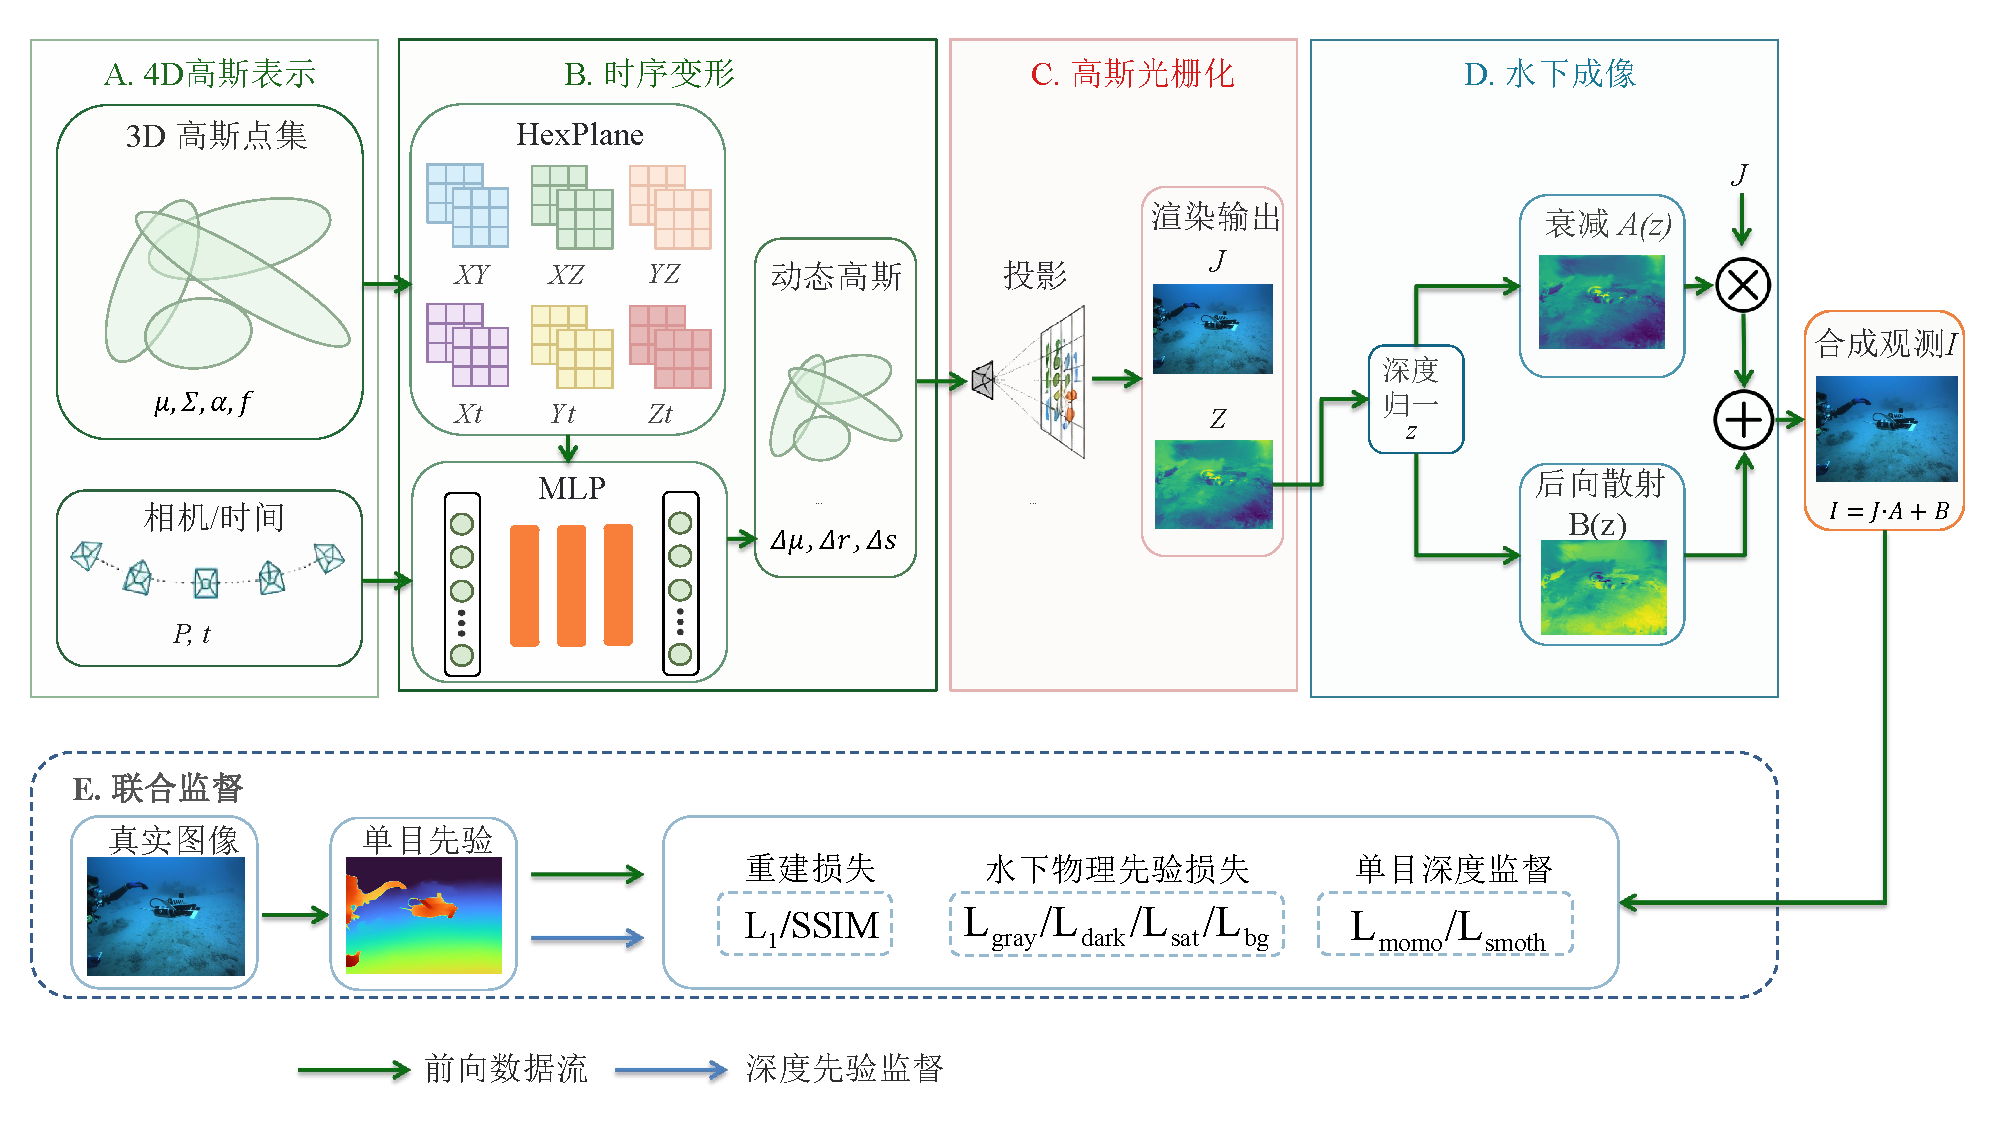
\includegraphics[width=\textwidth]{figures/pipeline.pdf}
  \caption{系统渲染管线。核心渲染流程以3D高斯点集为基础，经过变形网络调制后进行光栅化输出干净颜色图与深度图；水下成像模块基于渲染深度计算衰减与后向散射，并合成模拟观测图像；损失函数模块计算多项重建与物理先验损失，并将梯度回传至高斯参数和水下网络参数实现联合优化。}
  \label{fig:system_architecture}
\end{figure}

\textbf{（1）4D高斯点集。}场景由$N$个三维高斯椭球体参数化，每个高斯体携带位置$\boldsymbol{\mu} \in \mathbb{R}^3$、协方差$\boldsymbol{\Sigma} \in \mathbb{R}^{3\times3}$、不透明度$\alpha \in (0,1)$、球谐系数$\mathbf{f}$以及时间戳$t$\upcite{kerbl2023gaussian,wu2024gaussian}。

\textbf{（2）变形网络。}对于给定时刻$t$，多分辨率特征平面（HexPlane）与多层感知机（MLP）联合输出每个高斯体的位置增量$\Delta\boldsymbol{\mu}$、尺度增量$\Delta\mathbf{s}$和旋转增量$\Delta\mathbf{q}$，从而将规范空间中的高斯点云变形为当前帧的动态状态。

\textbf{（3）高斯光栅化。}经变形后的高斯点云通过可微分的基于分块排序的光栅化算法投影至图像平面，输出干净场景颜色图$\mathbf{J}$及深度图$\mathbf{Z}$。$\mathbf{J}$代表在无水体介质干扰时的真实辐射度。

\textbf{（4）水下成像模型。}将$\mathbf{J}$和$\mathbf{Z}$输入水下物理模型合成观测图像$\mathbf{I}$，逐通道形式为：
\begin{equation}
  I_c = J_c \cdot \exp\!\left(-\beta_c^D Z\right) + B_c^{\infty}\left(1 - \exp\!\left(-\beta_c^B Z\right)\right).
  \label{eq:uwmodel}
\end{equation}
其中，$\beta_c^D$为直接透射衰减系数，$B_c^{\infty}$为无穷远后向散射强度，$\beta_c^B$为后向散射衰减系数，均由水下网络预测。

\textbf{（5）联合优化。}将合成图像$\mathbf{I}$与真实观测图像$\mathbf{I}^{\mathrm{gt}}$进行对比，梯度同时回传至高斯参数和水下网络参数，实现联合优化。

\section{SeaSplat水下模块迁移}

\subsection{框架分析}

SeaSplat\upcite{seasplat2025icra}基于原始3DGS静态框架实现，而4DGS\upcite{wu2024gaussian}在其基础上引入了变形网络、多分辨率特征平面（HexPlane）及多分辨率哈希编码等核心组件，二者在接口设计与数据流结构上存在显著差异，迁移工作面临以下三个方面的挑战。

\textbf{渲染函数接口差异。}3DGS的渲染函数以静态高斯参数为输入，而4DGS在调用光栅化之前需先经过变形网络的时序处理，渲染函数扩展了时间戳和变形结果等额外参数。迁移时需将水下模块的介入点后移至光栅化之后，以确保输入给水下模型的颜色图$\mathbf{J}$是经过完整时序处理的干净渲染结果。

\textbf{优化器管理差异。}4DGS引入了多分辨率特征平面（HexPlane）参数和变形MLP参数两组新的可学习参数，其学习率调度策略与3DGS原有的高斯属性参数不同。本文未将水下模型参数并入原有高斯优化器，而是为后向散射网络和衰减网络分别建立独立优化器；训练时根据阶段选择执行水下优化器或高斯优化器的更新步骤，以避免两类参数的学习率调度和更新时机相互干扰。

\textbf{动态与静态表示差异。}SeaSplat假设场景静止，其推断的深度图在不同帧之间保持一致。引入4DGS后，每帧的高斯形态因变形网络而不同，导致深度图在时序上动态变化。水下物理模型必须以当前帧的实时渲染深度作为输入，而非预存的静态深度缓存。

综合考虑上述差异，迁移策略确定为在保持4DGS变形流程完全不变的前提下，在光栅化输出之后、损失计算之前插入水下成像模块实现功能集成。

\subsection{核心模块迁移}

本节给出本文从SeaSplat迁移并改写到4DGS渲染流程中的三个具体模块：后向散射网络（BackscatterNet）、直接透射衰减网络（AttenuateNet）以及四项水下专用损失函数。其中，参数初始化、独立优化器设置、阶段性更新控制以及对4DGS动态深度输入的适配均为本文针对动态框架进行的改写工作。

\textbf{后向散射网络（BackscatterNet）。}后向散射网络以归一化深度为输入，逐通道输出后向散射强度：
\begin{equation}
  B_c(Z) = \sigma(B_c^{\infty}) \cdot \left(1 - \exp(-\beta_c^B Z)\right).
  \label{eq:backscatter_impl}
\end{equation}网络结构为两层轻量卷积，参数量约1K，由独立的后向散射优化器更新。

\textbf{直接透射衰减网络（AttenuateNet）。}经消融对比，本文选用结构最简、训练更稳定的逐通道标量版本——每个通道学习一个标量衰减系数$\beta_c^D$：
\begin{equation}
  A_c(Z) = \exp\!\left(-\beta_c^D Z\right).
  \label{eq:attenuation_impl}
\end{equation}参数以较小正值初始化，使系统初始阶段接近无衰减状态，并由独立的衰减优化器更新，便于在精细阶段与后向散射网络同步完成水下物理分支的预热。

\textbf{损失函数迁移。}水下专用损失函数包含以下四个组件：

\begin{itemize}
  \item \textbf{暗通道先验损失}：基于He等人\upcite{he2011dcp}提出的暗通道先验，约束干净场景图像$\mathbf{J}$在局部窗口内至少有一个通道接近零，防止网络将水体散射残留嵌入干净图像；
  \item \textbf{灰世界先验损失}：约束干净图像每个颜色通道的均值趋向0.5，避免颜色通道间出现偏置性亮度不平衡；
  \item \textbf{RGB饱和度损失}：惩罚$\mathbf{J}$中超出$[0,1]$范围的像素值，维护物理合理性；
  \item \textbf{Alpha背景损失}：抑制相机前方水柱区域的高斯体不透明度，防止系统学习到虚假的水体填充体素，迁移过程中针对批尺寸$b=1$对掩码张量维度进行了专项修复。
\end{itemize}

\subsection{渲染流程}

在原有4DGS光栅化输出干净颜色$\mathbf{J}$和深度$\mathbf{Z}$之后，额外执行以下步骤，可参考图\ref{fig:system_architecture}的水下成像部分。

\textbf{步骤一：深度归一化。}将原始渲染深度归一化至$[0,1]$区间：
\begin{equation}
  \hat{\mathbf{Z}} = \frac{\mathbf{Z} - Z_{\min}}{Z_{\max} - Z_{\min} + \epsilon},
  \label{eq:depthnorm}
\end{equation}其中$Z_{\min}$、$Z_{\max}$为$\mathbf{Z}$的最小值与最大值。归一化可按帧动态计算或使用全局统计量；精细训练阶段采用帧级归一化以适应场景深度分布的动态变化。

\textbf{步骤二：水下网络前向传播。}将$\hat{\mathbf{Z}}$分别送入衰减与后向散射网络，按式\eqref{eq:attenuation_impl}与式\eqref{eq:backscatter_impl}逐元素得到衰减图$\mathbf{A}(\hat{\mathbf{Z}})$和后向散射图$\mathbf{B}(\hat{\mathbf{Z}})$。

\textbf{步骤三：水下成像合成。}按照式\eqref{eq:uwmodel}合成模拟水下图像$\mathbf{I}$：
\begin{equation}
  \mathbf{I} = \mathbf{J} \odot \mathbf{A}(\hat{\mathbf{Z}}) + \mathbf{B}(\hat{\mathbf{Z}}).
  \label{eq:synthesis}
\end{equation}其中$\odot$表示逐元素乘法。

上述过程整个合成路径完全可微，梯度可同时流向高斯点集参数和水下网络参数；实际参数更新则由训练阶段决定，如在水下预热阶段只更新后向散射与前向衰减参数。

\section{单目深度监督实现}

\subsection{深度图生成流程}

在水下动态重建中引入单目深度监督的思路最早由UDR-GS\upcite{udrgs2024symmetry}提出，用于缓解水下几何重建的深度歧义性。由于UDR-GS未提供开源代码，本节以Depth Anything V2\upcite{yang2024depthv2}为深度先验来源对该机制进行独立实现，并与本文迁移得到的水下物理模块及第\ref{sec:training-stages}节中的分阶段训练策略相耦合。Depth Anything V2在多种室内外场景上具备较好的跨域泛化能力，将其单目逆深度输出离线预处理后接入4DGS训练流程，能够满足实用需求。

深度图生成与处理流程如下：

（1）对数据集每张图像运行Depth Anything V2的前向推理，得到逆深度图（Inverse Depth Map）；

（2）将逆深度图归一化至$[0,255]$区间并保存为灰度图像。

选用逆深度而非线性深度的原因有以下两点：首先，水下远距离目标因散射效应造成视觉模糊，线性深度分布下远处区域的深度估计方差较大，逆深度变换可使近处高精度区域和远处区域在数值域中分布更为均匀；其次，逆深度与视差（Disparity）等价，在立体匹配和单目深度估计领域具有良好的物理解释性。

\subsection{监督机制}

\textbf{渲染深度获取。}在高斯光栅化过程中，深度图$\mathbf{Z}$通过复用颜色渲染的混合权重$w_i$对各高斯体中心深度进行加权累积得到：
\begin{equation}
  Z(\mathbf{p}) = \sum_{i} w_i(\mathbf{p}) \cdot z_i.
  \label{eq:renderdepth}
\end{equation}
其中，$\mathbf{p}$为像素坐标，$z_i$为第$i$个高斯体在相机坐标系下的深度值，$w_i(\mathbf{p})$与颜色渲染的混合权重共享，避免引入额外计算。

\textbf{尺度不确定性处理。}单目深度估计模型输出的深度图与真实度量深度之间存在未知的尺度与偏移不确定性。为消除该歧义，本文在计算损失前对渲染逆深度$d_{\mathrm{render}}$和单目逆深度$d_{\mathrm{mono}}$均进行基于均值$\mu_d$和标准差$\sigma_d$的归一化处理：
\begin{equation}
  \tilde{d} = \frac{d - \mu_d}{\sigma_d + \epsilon}.
  \label{eq:depthnorm2}
\end{equation}其中$\mu_d$表示深度图$d$在所有像素上的均值，$\sigma_d$表示对应的标准差，$\epsilon$为防止除零的小常数。此归一化操作使损失对绝对尺度不敏感，仅约束深度图的相对结构（即深度梯度与相对远近关系）与单目先验保持一致。

\textbf{损失函数。}在获得归一化逆深度后，沿用UDR-GS的整体思路，本文不直接对原始深度值施加强约束，而是将单目深度作为描述场景相对几何结构的软监督信号。具体而言，单目深度监督损失定义为归一化逆深度图之间的加权L1距离：
\begin{equation}
  \mathcal{L}_{\mathrm{mono}} =
  \frac{\sum_{\mathbf{p}} \alpha(\mathbf{p})
  \left|\tilde{d}_{\mathrm{render}}(\mathbf{p}) - \tilde{d}_{\mathrm{mono}}(\mathbf{p})\right|}
  {\sum_{\mathbf{p}} \alpha(\mathbf{p}) + \epsilon}.
  \label{eq:depthloss}
\end{equation}其中，$\alpha(\mathbf{p}) \in [0,1]$为像素$\mathbf{p}$处的高斯累积透明度，对高斯覆盖良好的区域给予更高监督权重，对空白背景区域减少干扰；分母中的$\sum_{\mathbf{p}}\alpha(\mathbf{p})+\epsilon$用于对有效监督区域进行归一化，使不同视角、不同前景覆盖面积下的损失幅值保持相对稳定。采用逆深度形式的原因在于，近景区域对新视角合成中的遮挡关系和局部几何误差更为敏感，逆深度能够在数值上增强近处结构的约束；同时，均值方差归一化消除了Depth Anything V2预测结果中的全局尺度和偏移不确定性，使该损失主要关注物体轮廓、深度层次和相对远近关系，而不强制渲染深度与单目估计在绝对尺度上一致。该损失与光度重建损失共同作用：光度项约束图像颜色一致性，单目深度项则抑制水下散射、低纹理区域和动态扰动造成的高斯漂浮与局部深度塌缩，从而提升高斯场景表示的几何稳定性。

\textbf{配置参数。}实现中需要指定单目深度先验的存放目录，并声明预存文件为逆深度格式，同时启用单目深度监督开关。深度监督损失权重$\lambda_{\mathrm{mono}}$设定为0.1，并配合热启动调度策略在训练初期逐步引入。

\section{分阶段训练策略}
\label{sec:training-stages}

分阶段训练策略用于降低多组件联合优化的不稳定性。当水下网络、变形网络与高斯点集同时从零开始优化时，颜色退化、几何误差和动态形变误差会在同一光度损失中相互干扰：水下网络若过早引入，可能把几何错位解释为后向散射或衰减；变形网络若在几何尚未稳定时充分更新，则容易把水体造成的颜色差异误当作运动信号。为此，本文不直接启动全部模块，而是先优化几何结构，再使用独立优化器预热水下分支，最后交替控制高斯参数与后向散射与前向衰减参数的更新。

本文的训练流程继承了4DGS\upcite{wu2024gaussian}原有的两阶段框架：粗训练阶段在不开启水下物理模型的条件下与原始4DGS等价，用于建立基础几何结构；精细训练阶段则启用水下模块、深度监督等本文新增的组件。本文的工作集中于精细训练阶段，针对水下网络、动态高斯属性与深度监督之间的梯度耦合，将其进一步细分为"后向散射与前向衰减参数预热—高斯颜色调整—联合训练"三个子阶段，并在联合训练阶段交替更新高斯参数和水下模块。实现中通过跳过高斯优化器步骤，使预热和间歇式专项更新只作用于后向散射网络与衰减网络。完整的阶段划分及各阶段中的可学习参数与损失项配置如图\ref{fig:training_stages}所示。

阶段划分对应三类优化对象的启停边界：高斯几何与密度控制首先建立可渲染的基础结构；水下参数随后在固定几何上估计衰减和后向散射的量级；高斯颜色再在相对稳定的水下参数下校准到干净外观空间；最后进入联合训练，交替更新高斯参数和水下模块。该策略本质上是训练稳定性设计。

\begin{figure}[htbp]
  \centering
  \begin{tikzpicture}[
  font=\footnotesize,
  >=Stealth,
  stage/.style={
    draw=#1!75!black,
    fill=#1!12,
    rounded corners=2pt,
    line width=0.7pt,
    minimum height=1.0cm,
    text width=2.6cm,
    align=center,
    inner sep=4pt
  },
  stage/.default=orange,
  group/.style={
    draw=#1!70!black,
    dashed,
    rounded corners=4pt,
    line width=0.6pt,
    inner sep=8pt
  },
  note/.style={font=\scriptsize, align=center, text=black!75},
  arr/.style={->, line width=0.75pt, draw=black!70}
]

% ===== Stage row =====
\node[stage=cyan]   (s1)                       {粗训练阶段\\\scriptsize iter 0--3000};
\node[stage=orange, right=0.6cm of s1] (s2)    {BS/AT 预热\\\scriptsize iter 3000--4000};
\node[stage=red,    right=0.6cm of s2] (s3)    {高斯颜色调整\\\scriptsize iter 4000--6000};
\node[stage=purple, right=0.6cm of s3] (s4)    {联合训练\\\scriptsize iter 6000--20000};

\draw[arr] (s1) -- (s2);
\draw[arr] (s2) -- (s3);
\draw[arr] (s3) -- (s4);

% ===== Key annotation under each stage =====
\node[note, below=0.15cm of s1] {更新高斯几何与颜色\\水下模块未启用};
\node[note, below=0.15cm of s2] {更新BS/AT\\冻结高斯几何与颜色};
\node[note, below=0.15cm of s3] {仅更新高斯颜色\\冻结高斯几何与BS/AT};
\node[note, below=0.15cm of s4] {全参数联合更新\\并间歇式专项更新 BS/AT };

% ===== Group framing =====
\begin{scope}[on background layer]
  \node[group=cyan, fit=(s1)] (g1) {};
  \node[group=orange, fit=(s2)(s3)(s4)] (g2) {};
\end{scope}

\node[note, text=cyan!55!black, above=0.05cm of g1.north]   {粗阶段};
\node[note, text=orange!55!black, above=0.05cm of g2.north] {精细阶段子流程};

\end{tikzpicture}

  \caption{分阶段训练策略流程图。最外层的粗训练与精细训练两段框架继承自4DGS（蓝色虚线框），本文在精细训练阶段内部进一步细分出后向散射与前向衰减参数预热、高斯颜色调整与联合训练三个子阶段（橙色虚线框），并在联合训练阶段引入间歇式专项更新。}
  \label{fig:training_stages}
\end{figure}

\subsection{粗训练阶段}

该阶段位于训练流程的起始部分，在水下物理模型尚未激活的条件下，系统等价于原始 4DGS 训练，用于建立场景的基础几何骨架。损失函数为：
\begin{equation}
  \mathcal{L}_{\mathrm{coarse}} = (1-\lambda_{\mathrm{s}})\mathcal{L}_1(\mathbf{J}, \mathbf{I}^{\mathrm{gt}}) + \lambda_{\mathrm{s}} \mathcal{L}_{\mathrm{D}\mbox{-}\mathrm{SSIM}}(\mathbf{J}, \mathbf{I}^{\mathrm{gt}}).
  \label{eq:losscoarse}
\end{equation}
其中，$\lambda_{\mathrm{s}}=0.2$为结构损失权重，$\mathcal{L}_{\mathrm{D}\mbox{-}\mathrm{SSIM}}$表示由SSIM构造的结构差异项。此阶段开启自适应密度控制（Adaptive Density Control），执行高斯体的分裂、克隆与修剪操作，建立场景的基础几何骨架。为避免视角相关颜色效应与后续水下模型产生干扰，球谐阶数固定为0，使每个高斯体只学习与视角无关的漫反射颜色。

\subsection{精细阶段初始化}

在粗训练完成之时，系统执行一次性的精细阶段初始化，该阶段在图\ref{fig:training_stages}未显示：创建并启用后向散射网络与衰减网络，并分别为二者建立优化器。选用粗训练阶段学习到的背景颜色对后向散射网络的$B^{\infty}$参数进行初始化，使其从一个合理的先验值起步，加速精细阶段的收敛。

在初始化完成的第一个迭代步内，高斯体的位置、不透明度、缩放、旋转和颜色参数被临时冻结，防止刚启用水下模型时不稳定的梯度影响几何结构；下一迭代步起即解冻后向散射与前向衰减参数进入预热阶段。

\subsection{后向散射与前向衰减参数预热阶段}

该阶段冻结高斯点集所有参数，仅执行后向散射与前向衰减参数的更新，在高斯几何不受干扰的条件下，让水下物理模型快速捕捉水体介质的光学特性（各通道衰减系数的量级与后向散射基准强度），为后续联合优化提供稳定的水下模型初始化。此时损失仍由图像重建项和水下相关约束共同决定，但高斯优化器不执行更新。

\subsection{高斯颜色调整阶段}

水下物理模型预热完成后，切换至高斯颜色调整阶段，暂停后向散射与前向衰减参数更新，转而执行高斯颜色参数更新，用于校准高斯点集的颜色属性。其目的在于，在水下网络基本确定水体介质参数的前提下，让高斯颜色在去水体后的干净颜色空间中重新校准，使$\mathbf{J}$逐步逼近真实物体的本征颜色，而非被水体污染的表观颜色。

\subsection{联合训练阶段}

在高斯颜色完成初步对齐后，训练进入末段的联合训练阶段：高斯点集与水下物理模型的参数交替更新：

\begin{itemize}
  \item 在每个完整更新周期内，按预设比例插入若干步的水下物理模型专项更新，此时只执行后向散射与衰减参数的更新步骤，并跳过高斯参数更新；
  \item 其余迭代步执行高斯优化器步骤，并跳过水下参数更新，使动态高斯表示继续根据重建损失和深度监督进行调整。
\end{itemize}

该机制的物理动机是，随着场景几何的持续改变（高斯点云的位置和密度在联合优化中仍会变化），渲染深度图$\mathbf{Z}$也随之改变，需要定期给水下网络提供独立的优化机会，使其适应几何变化。

完整损失函数在该阶段激活全部组件：
\begin{equation}
  \begin{aligned}
    \mathcal{L} =\ & \mathcal{L}_1 + \lambda_{\mathrm{s}}\mathcal{L}_{\mathrm{D}\mbox{-}\mathrm{SSIM}}
                  + \lambda_{\mathrm{smooth}}\mathcal{L}_{\mathrm{smooth}}
                  + \lambda_{\mathrm{dark}}\mathcal{L}_{\mathrm{dark}} \\
                & + \lambda_{\mathrm{gray}}\mathcal{L}_{\mathrm{gray}}
                  + \lambda_{\mathrm{sat}}\mathcal{L}_{\mathrm{sat}}
                  + \lambda_{\mathrm{bg}}\mathcal{L}_{\mathrm{bg}}
                  + \lambda_{\mathrm{mono}}\mathcal{L}_{\mathrm{mono}}.
  \end{aligned}
  \label{eq:lossfull}
\end{equation}
各损失项含义如下：$\mathcal{L}_1$为像素级L1重建损失；$\mathcal{L}_{\mathrm{D}\mbox{-}\mathrm{SSIM}}$为由结构相似性指数\upcite{wang2004ssim}构造的结构差异损失；$\mathcal{L}_{\mathrm{smooth}}$为深度平滑正则项，约束渲染深度图在空间上的平滑性；$\mathcal{L}_{\mathrm{dark}}$为暗通道先验损失\upcite{he2011dcp}；$\mathcal{L}_{\mathrm{gray}}$为灰世界先验损失；$\mathcal{L}_{\mathrm{sat}}$为RGB饱和度损失；$\mathcal{L}_{\mathrm{bg}}$为Alpha背景损失；$\mathcal{L}_{\mathrm{mono}}$为单目深度监督损失（式\eqref{eq:depthloss}）。

为防止训练初期损失震荡，各辅助损失项采用线性热启动（Warm-Up）调度策略：
\begin{equation}
  w(k) = w_{\mathrm{base}} \cdot \max\!\left(0,\; \min\!\left(1,\; \frac{k - k_{\mathrm{start}}}{k_{\mathrm{ramp}}}\right)\right).
  \label{eq:warmup}
\end{equation}
其中，$k$为当前迭代步，$k_{\mathrm{start}}$为该损失项的激活步，$k_{\mathrm{ramp}}$为热启动步数（默认500步）。

\section{本章小结}

本章详细介绍了面向扰动水下环境的新视角合成系统的完整设计与实现。主要内容包括：（1）以4DGS为骨架、SeaSplat水下物理模型为外层包装、Depth Anything V2为深度先验的三层系统架构设计；（2）SeaSplat核心水下模块（后向散射网络、衰减网络及多项水下专用损失）向4DGS框架的迁移方案；（3）借鉴UDR-GS将单目深度先验融入水下动态重建的思路，由于UDR-GS未开源，本文以Depth Anything V2为深度源对该机制进行了独立实现并处理了尺度不确定性；（4）在4DGS自身粗-精二段框架之上，针对精细阶段内部多组件梯度干扰所设计的子阶段训练策略。

\chapter{实验结果与分析}

\section{实验设置}

\subsection{实验环境}

本文所有实验均在同一硬件平台上完成，具体配置如表\ref{tab:hardware}所示。

\begin{table}[htbp]
  \centering
  \tablecaption{实验硬件与软件环境配置}
  \label{tab:hardware}
  \resizebox{\textwidth}{!}{%
  \begin{tabular}{lll}
    \hline
    \textbf{类别} & \textbf{配置项} & \textbf{具体参数} \\
    \hline
    \multirow{3}{*}{硬件环境} & 处理器（CPU） & Intel Core i9-14900HX \\
                               & 图形处理器（GPU） & NVIDIA GeForce RTX 4060 Laptop（8GB显存） \\
                               & 内存（RAM） & 32GB DDR5 \\
    \hline
    \multirow{3}{*}{软件环境} & 操作系统 & Windows 11 专业版 \\
                               & CUDA版本 & CUDA 11.8 \\
                               & 深度学习框架 & PyTorch 2.5.1 \\
    \hline
  \end{tabular}%
  }
\end{table}



\subsection{数据集}

为全面评估所提方法在不同水下场景条件下的性能，本文采用两类数据集进行实验，分别覆盖动态水下场景与静态水下场景。

\textbf{（1）动态水下场景数据集}

动态水下场景实验采用UDR-GS\upcite{udrgs2024symmetry}所提供的四个数据子集，每个子集均包含若干连续帧的水下视频图像，具体包括：

\begin{itemize}
  \item \textbf{Robot}：水下机械臂操作场景，共34帧，分辨率为$800\times600$像素。机械臂的往复运动引入了规律性的刚体动态，是测试动态建模精度的典型场景。
  \item \textbf{Fish}：水下鱼类游动场景，记录了多条鱼在珊瑚礁附近自由游动的过程。鱼体的非刚性快速运动对动态建模提出了较高要求。
  \item \textbf{Coral}：珊瑚礁随水流摆动场景，呈现出软体珊瑚枝条在水流驱动下的周期性缓慢摆动，是典型的连续形变动态场景。
  \item \textbf{Streaks}：水下光线焦散或光纹场景，由水面折射形成的动态光纹投影于水底，光斑形状随时间不断变化，对场景外观建模构成挑战。
\end{itemize}

图\ref{fig:dynamic_dataset_samples}展示了四个动态水下场景数据集的示例图像。

\begin{figure}[htbp]
  \centering
  \setlength{\tabcolsep}{2pt}
  \begin{tabular}{cccc}
    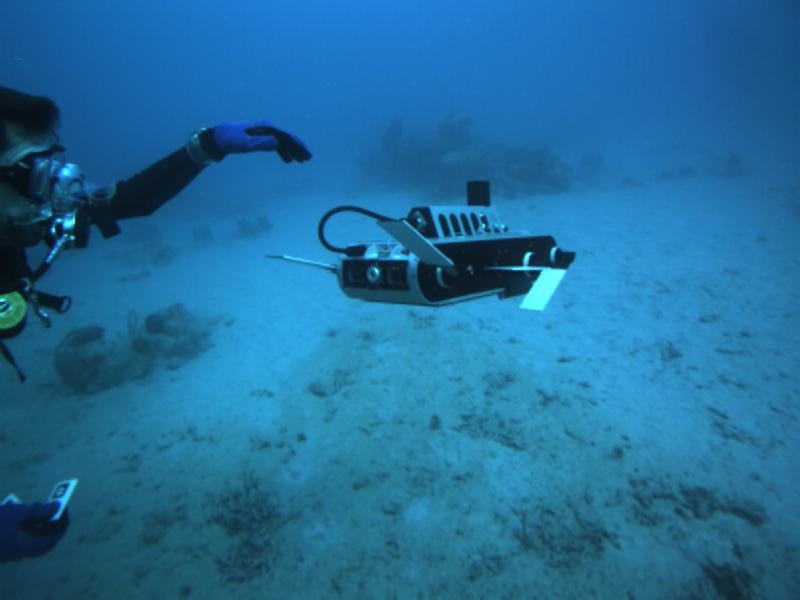
\includegraphics[width=0.23\textwidth]{figures/dataset_samples/robot_sample.jpg} &
    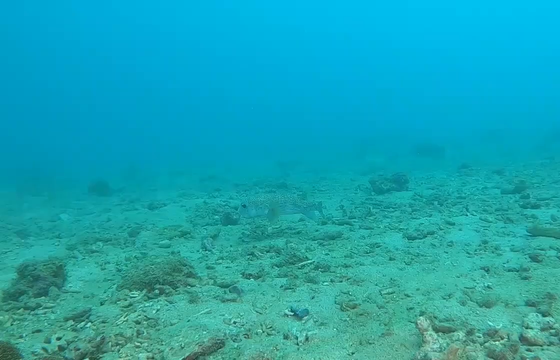
\includegraphics[width=0.23\textwidth]{figures/dataset_samples/fish_sample.png} &
    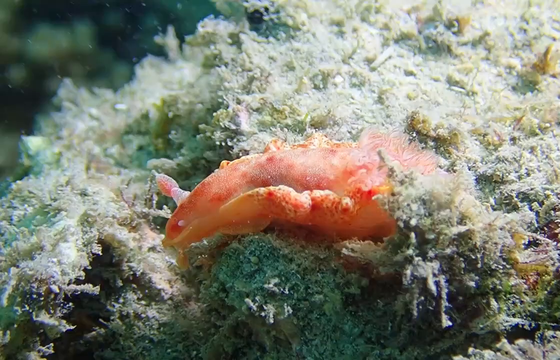
\includegraphics[width=0.23\textwidth]{figures/dataset_samples/coral_sample.png} &
    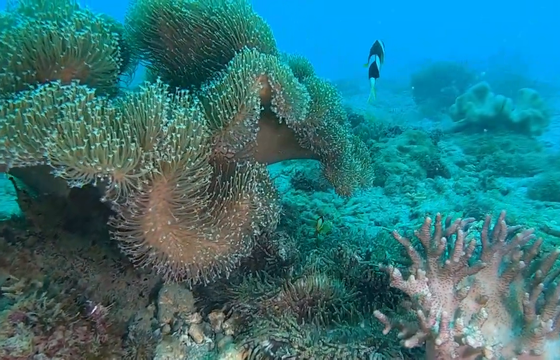
\includegraphics[width=0.23\textwidth]{figures/dataset_samples/streaks_sample.png} \\
    (a) Robot & (b) Fish & (c) Coral & (d) Streaks \\
  \end{tabular}
  \caption{动态水下场景数据集示例图像。(a) Robot：水下机械臂操作场景；(b) Fish：鱼类游动场景；(c) Coral：珊瑚摆动场景；(d) Streaks：水下光纹场景。}
  \label{fig:dynamic_dataset_samples}
\end{figure}

\textbf{（2）静态水下场景数据集}

静态水下场景实验采用SeaThru-NeRF数据集，包含四个典型水下拍摄地点：

\begin{itemize}
  \item \textbf{Curasao}：加勒比海库拉索岛近岸礁盘场景，水体清澈，色偏程度中等。
  \item \textbf{IUI3-RedSea}：红海水下研究站附近场景，水体可见度较高，场景包含丰富的珊瑚与礁石结构。
  \item \textbf{JapaneseGardens-RedSea}：红海Japanese Gardens珊瑚礁场景，细粒度纹理丰富，适合检验方法在复杂静态结构下的外观建模能力。
  \item \textbf{Panama}：巴拿马热带海域场景，水体略浑浊，散射效应相对明显。
\end{itemize}

图\ref{fig:static_dataset_samples}展示了SeaThru-NeRF数据集中四个静态水下场景的示例图像。

\begin{figure}[htbp]
  \centering
  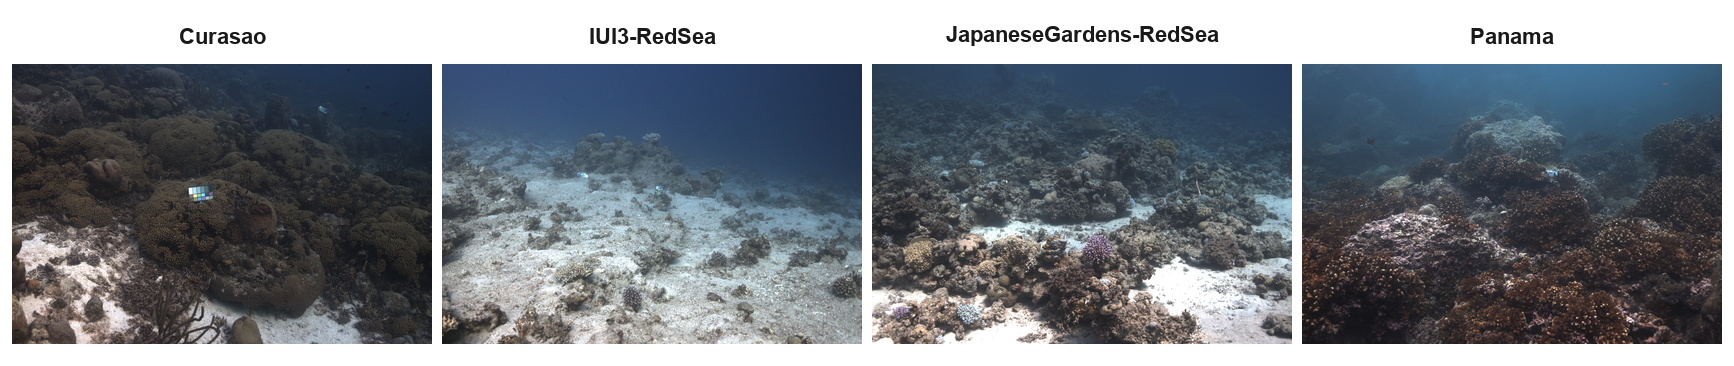
\includegraphics[width=\textwidth]{figures/dataset_samples/static_seathru_samples.png}
  \caption{SeaThru-NeRF静态水下场景数据集示例图像。四个子图依次对应Curasao、IUI3-RedSea、JapaneseGardens-RedSea与Panama场景。}
  \label{fig:static_dataset_samples}
\end{figure}

上述数据集的组合能够有效检验所提方法在处理动态运动、水下色偏与散射等多种挑战时的综合性能。

\subsection{评估指标}

本文采用以下三项广泛使用的图像质量评估指标对各方法进行定量评价。

\textbf{（1）峰值信噪比（PSNR）}

峰值信噪比（Peak Signal-to-Noise Ratio，PSNR）是衡量像素级重建精度的经典指标，其定义为：

\begin{equation}
  \mathrm{PSNR} = 10 \cdot \log_{10} \left( \frac{L^2}{\mathrm{MSE}} \right).
  \label{eq:psnr}
\end{equation}
其中，$L$为像素最大值；若图像归一化至$[0,1]$，则$L=1$，若在8位像素空间计算，则$L=255$；$\mathrm{MSE}$为均方误差。PSNR以分贝（dB）为单位，数值越高表示渲染图像与真实图像在像素层面的偏差越小，重建精度越高。

\textbf{（2）结构相似性指数（SSIM）}

结构相似性指数（Structural Similarity Index，SSIM）\upcite{wang2004ssim}从亮度、对比度与结构三个维度综合衡量图像质量，比PSNR更接近人类视觉感知特性，取值范围为$[0,1]$，数值越接近1表示感知质量越好。

\textbf{（3）感知图像块相似度（LPIPS）}

感知图像块相似度（Learned Perceptual Image Patch Similarity，LPIPS）\upcite{zhang2018lpips}利用预训练深度神经网络提取的高层语义特征计算图像间的感知距离。与PSNR和SSIM不同，LPIPS数值越低表示渲染结果与参考图像在感知质量上越接近，更能反映人类对图像细节与纹理质量的主观判断。

\subsection{对比方法}

为全面评估所提方法的性能，本文选取以下四种具有代表性的基线方法进行对比：

\begin{itemize}
  \item \textbf{3DGS}：原始三维高斯溅射方法\upcite{kerbl2023gaussian}，不包含水下物理模型，也不具备动态场景建模能力，作为基础基线。
  \item \textbf{4DGS}：四维高斯溅射方法\upcite{wu2024gaussian}，通过引入时间维度扩展实现动态场景建模，但不包含水下物理退化模型，代表动态重建的主流基线。
  \item \textbf{SeaSplat}：静态水下高斯溅射方法\upcite{seasplat2025icra}，将水下物理成像模型集成至3DGS框架，能够处理色偏与散射问题，但仅针对静态场景设计，代表静态水下重建基线。
  \item \textbf{UDR-GS}：基于深度正则化的动态水下高斯溅射方法\upcite{udrgs2024symmetry}，同时具备动态建模与水下图像处理能力。
\end{itemize}



\section{动态场景实验结果}

\subsection{定量实验分析}

表\ref{tab:psnr_dynamic}给出了各方法在四个动态水下场景上的PSNR（单位：dB）定量对比结果。每列最优值以\textbf{粗体}标注。

\begin{table}[htbp]
  \centering
  \tablecaption{各方法在动态水下场景上的PSNR对比（单位：dB，越高越好）}
  \label{tab:psnr_dynamic}
  \begin{tabular}{lccccc}
    \hline
    \textbf{方法} & \textbf{Robot} & \textbf{Fish} & \textbf{Coral} & \textbf{Streaks} & \textbf{平均值} \\
    \hline
    3DGS\upcite{kerbl2023gaussian}       & 28.59 & 24.66 & 26.78 & 26.47 & 26.63 \\
    4DGS\upcite{wu2024gaussian}          & 29.49 & 29.09 & 31.14 & 28.81 & 29.63 \\
    UDR-GS\upcite{udrgs2024symmetry}     & 29.62 & \textbf{29.24} & 32.43 & 28.91 & 30.05 \\
    SeaSplat\upcite{seasplat2025icra}    & 28.21 & 23.30 & 26.58 & 26.16 & 26.06 \\
    \textbf{本文方法}                    & \textbf{29.71} & 28.52 & \textbf{33.29} & \textbf{30.65} & \textbf{30.54} \\
    \hline
  \end{tabular}
\end{table}

由表\ref{tab:psnr_dynamic}可以得出以下结论：

\textbf{第一}，本文方法在四个动态场景中的三个（Robot、Coral、Streaks）均取得最优PSNR，平均PSNR为30.54 dB，相较于最接近的基线UDR-GS（30.05 dB）提升约1.6\%，相较于4DGS（29.63 dB）提升约3.1\%，展现出所提方法在动态水下场景上的综合优势。

\textbf{第二}，在Fish场景中，本文方法（28.52 dB）略低于UDR-GS（29.24 dB），差距约为2.5\%。分析认为，Fish场景中鱼体运动速度快且无规律性，快速运动区域的颜色信息在多帧间变化剧烈，水下颜色恢复模块在此类场景中与动态建模模块存在一定程度的梯度干扰，导致两者联合优化时出现轻微的性能损失。UDR-GS专注于几何一致性建模，不引入颜色恢复的额外约束，因此在该场景上表现更为稳定。

\textbf{第三}，两种静态方法（3DGS与SeaSplat）在所有动态场景上均明显落后于动态方法，证明动态建模能力对于处理含运动元素的水下场景至关重要。

\textbf{多指标综合对比。}为进一步评估各方法的感知质量，表\ref{tab:multi_metric}给出了本文方法与基线UDR-GS在四个动态场景上的PSNR、SSIM与LPIPS三项指标的综合对比。

\begin{table}[htbp]
  \centering
  \tablecaption{本文方法与UDR-GS在动态场景上的多指标综合对比}
  \label{tab:multi_metric}
  \begin{tabular}{lcccccc}
    \hline
    \multirow{2}{*}{\textbf{场景}} & \multicolumn{3}{c}{\textbf{本文方法}} & \multicolumn{3}{c}{\textbf{UDR-GS\upcite{udrgs2024symmetry}}} \\
    \cline{2-7}
    & PSNR$\uparrow$ & SSIM$\uparrow$ & LPIPS$\downarrow$ & PSNR$\uparrow$ & SSIM$\uparrow$ & LPIPS$\downarrow$ \\
    \hline
    Robot   & \textbf{29.71} & \textbf{0.9387} & 0.1587          & 29.62 & 0.9312 & \textbf{0.0840} \\
    Fish    & 28.52          & 0.8218          & \textbf{0.1374} & \textbf{29.24} & \textbf{0.8231} & 0.1514 \\
    Coral   & \textbf{33.29} & \textbf{0.9640} & 0.0493          & 32.43 & 0.9475 & \textbf{0.0479} \\
    Streaks & \textbf{30.65} & \textbf{0.9349} & \textbf{0.0605} & 28.91 & 0.8648 & 0.0883 \\
    \hline
  \end{tabular}
\end{table}

综合三项指标可以观察到：在Robot与Coral场景中，本文方法在PSNR和SSIM上均优于UDR-GS，但LPIPS略高；在Streaks场景中，本文方法在全部三项指标上均明显优于UDR-GS，PSNR提升1.74 dB（+6.0\%），SSIM提升0.0701（+8.1\%），LPIPS降低0.0278（$-$31.5\%），提升幅度最为显著；在Fish场景中，本文方法LPIPS更低（0.1374 vs 0.1514），即感知质量更优，但PSNR与SSIM略逊。

\section{静态水下场景实验结果}

为进一步评估本文方法在静态水下场景上的迁移能力，本文在SeaThru-NeRF\upcite{levy2023seathrunerf}数据集所提供的四个典型水下场景上进行实验，包括Curaçao、IUI3-RedSea、JapaneseGardens-RedSea与Panama。对比方法包括原始3DGS\upcite{kerbl2023gaussian}、SeaThru-NeRF\upcite{levy2023seathrunerf}（下表中简记为STN）、SeaSplat\upcite{seasplat2025icra}以及未引入水下物理模型的原始4DGS\upcite{wu2024gaussian}。其中3DGS、4DGS、STN与SeaSplat的指标取自SeaSplat论文公开报告。表\ref{tab:psnr_static}给出了PSNR/SSIM/LPIPS三项指标的综合对比，每行最优值以\textbf{粗体}标注。

\begin{table}[htbp]
  \centering
  \tablecaption{静态水下场景（SeaThru-NeRF\upcite{levy2023seathrunerf}数据集）多方法定量对比（PSNR$\uparrow$ / SSIM$\uparrow$ / LPIPS$\downarrow$）}
  \label{tab:psnr_static}
  \resizebox{\textwidth}{!}{%
  \begin{tabular}{lccccc}
    \hline
    \textbf{场景} & \textbf{3DGS}\upcite{kerbl2023gaussian} & \textbf{STN}\upcite{levy2023seathrunerf} & \textbf{SeaSplat}\upcite{seasplat2025icra} & \textbf{4DGS}\upcite{wu2024gaussian} & \textbf{本文方法} \\
    \hline
    Curaçao                & 28.01 / 0.88 / 0.21          & 30.08 / 0.87 / 0.27 & \textbf{30.30 / 0.90 / 0.19} & 28.05 / 0.75 / 0.40 & 28.82 / 0.77 / 0.26 \\
    IUI3-RedSea            & 21.11 / 0.81 / 0.29          & 26.01 / 0.79 / 0.32 & \textbf{26.67 / 0.87 / 0.21} & 24.43 / 0.68 / 0.41 & 25.27 / 0.72 / 0.34 \\
    JapaneseGardens-RedSea & 21.47 / 0.85 / 0.22          & 21.74 / 0.77 / 0.29 & 22.70 / \textbf{0.87 / 0.18} & 21.81 / 0.76 / 0.33 & \textbf{23.38} / 0.81 / 0.24 \\
    Panama                 & \textbf{29.64 / 0.90} / 0.17 & 27.69 / 0.83 / 0.28 & 28.76 / \textbf{0.90 / 0.15} & 25.63 / 0.75 / 0.37 & 26.86 / 0.80 / 0.33 \\
    \hline
  \end{tabular}%
  }
\end{table}

为进一步从视觉层面对静态场景结果进行比较，图\ref{fig:static_multimethod_curacao}至图\ref{fig:static_multimethod_panama}给出了五种方法在四个SeaThru-NeRF场景上的代表性渲染结果及对应深度图。每幅图对应一个数据集，列方向依次为3DGS、SeaThru-NeRF（STN）、SeaSplat、4DGS与本文方法，上行为渲染结果，下行为深度图。由于整理得到的3DGS结果未包含对应深度输出，图中以N/A标记。

\begin{figure}[htbp]
  \centering
  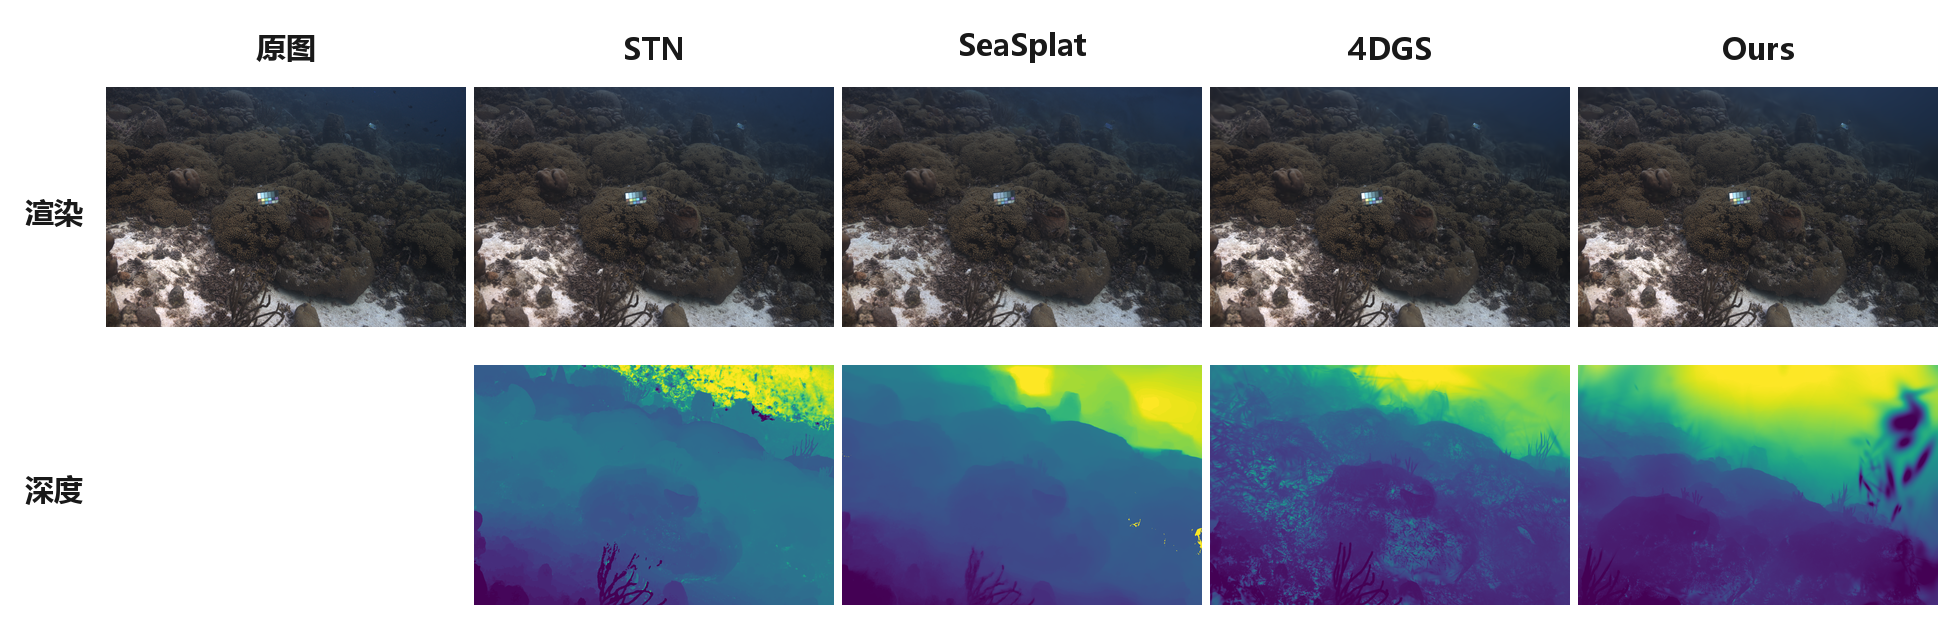
\includegraphics[width=\textwidth]{figures/static_multimethod/curacao_static_models_depth.png}
  \caption{Curaçao场景五种方法渲染结果与深度图对比。}
  \label{fig:static_multimethod_curacao}
\end{figure}

\begin{figure}[htbp]
  \centering
  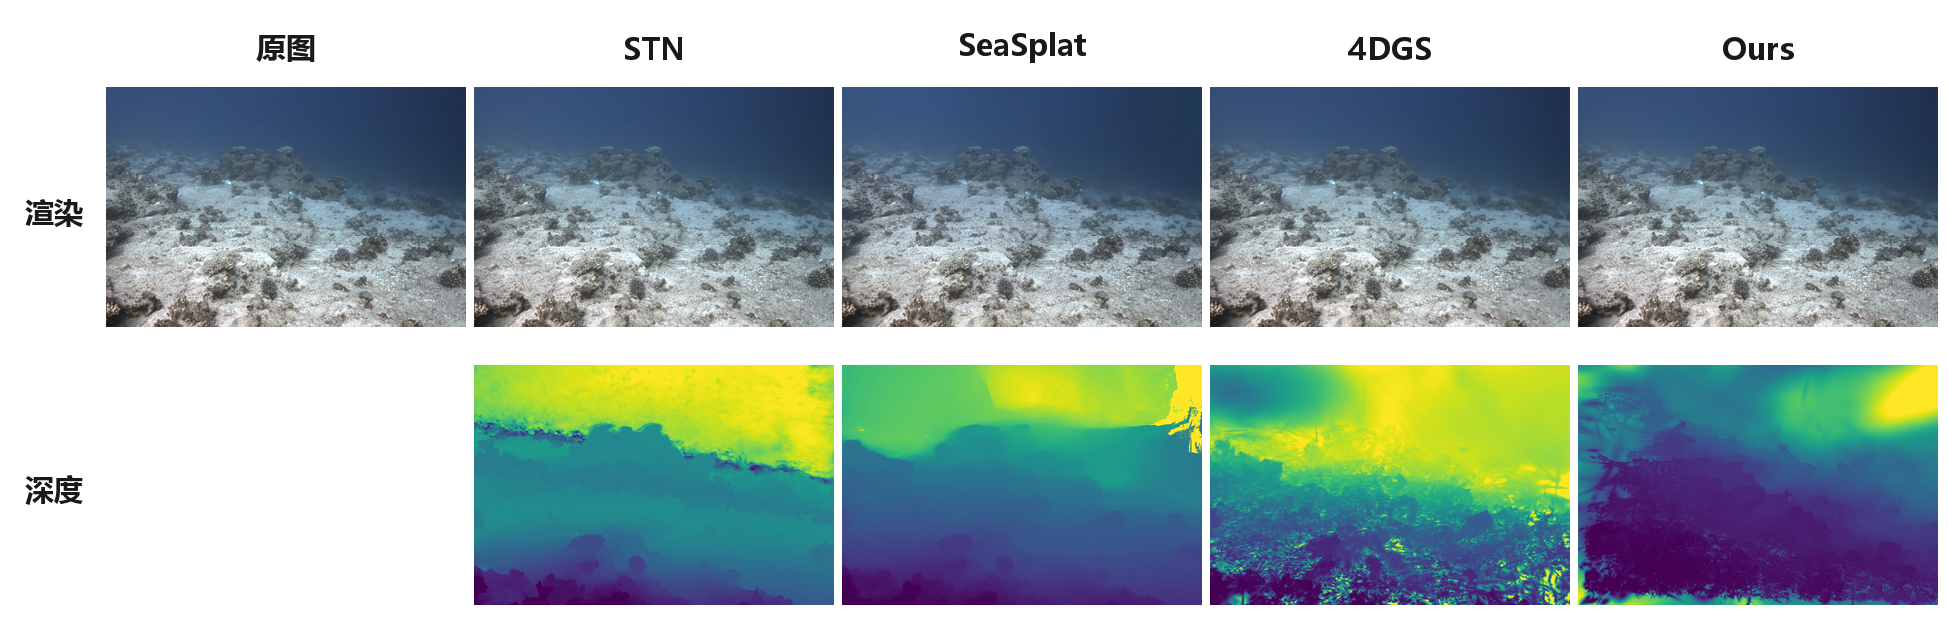
\includegraphics[width=\textwidth]{figures/static_multimethod/iui3_redsea_static_models_depth.png}
  \caption{IUI3-RedSea场景五种方法渲染结果与深度图对比。}
  \label{fig:static_multimethod_iui3}
\end{figure}

\begin{figure}[htbp]
  \centering
  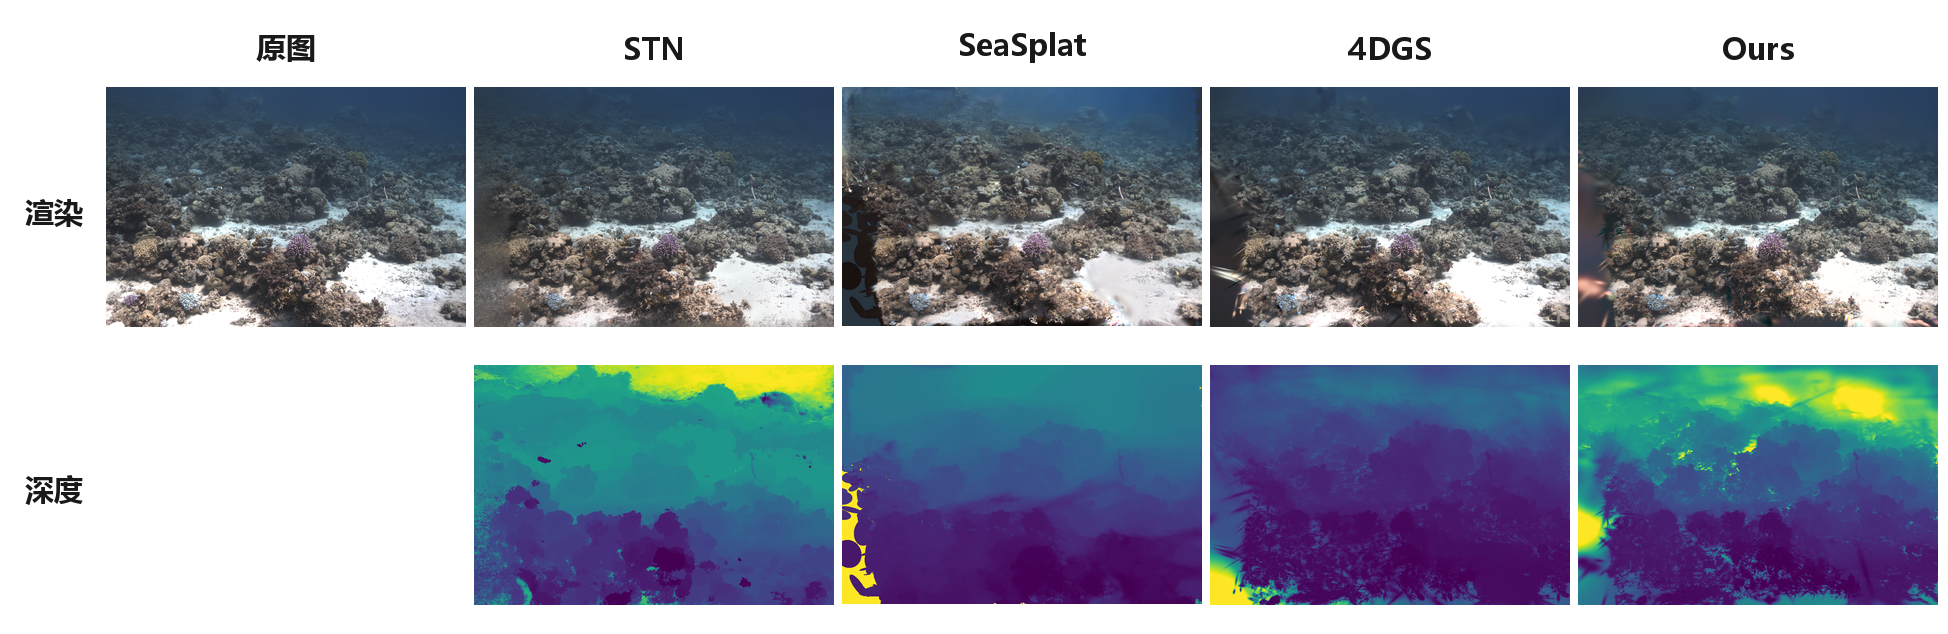
\includegraphics[width=\textwidth]{figures/static_multimethod/japanese_gardens_static_models_depth.png}
  \caption{JapaneseGardens-RedSea场景五种方法渲染结果与深度图对比。}
  \label{fig:static_multimethod_japanese}
\end{figure}

\begin{figure}[htbp]
  \centering
  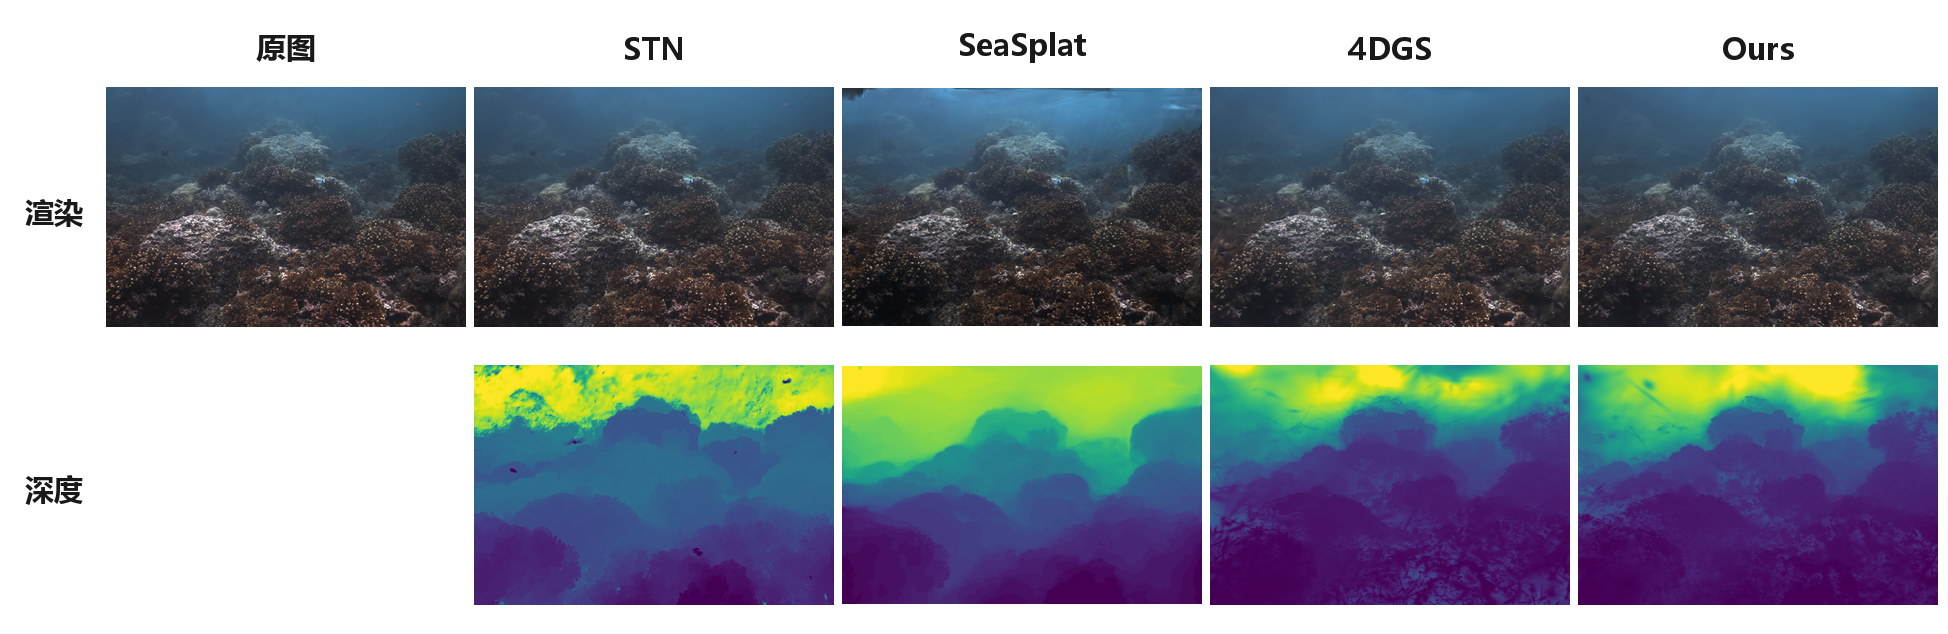
\includegraphics[width=\textwidth]{figures/static_multimethod/panama_static_models_depth.png}
  \caption{Panama场景五种方法渲染结果与深度图对比。}
  \label{fig:static_multimethod_panama}
\end{figure}

\subsection{JapaneseGardens-RedSea渲染与去水结果}

为进一步展示静态复杂珊瑚礁场景中的外观恢复效果，图\ref{fig:static_japanese_dewater}给出了JapaneseGardens-RedSea场景的原图、渲染结果与去水结果。图中列方向依次为原始水下图像、SeaThru-NeRF、SeaSplat与本文方法；行方向分别对应带水渲染结果与依据水下成像模型反演得到的去水结果。

\begin{figure}[htbp]
  \centering
  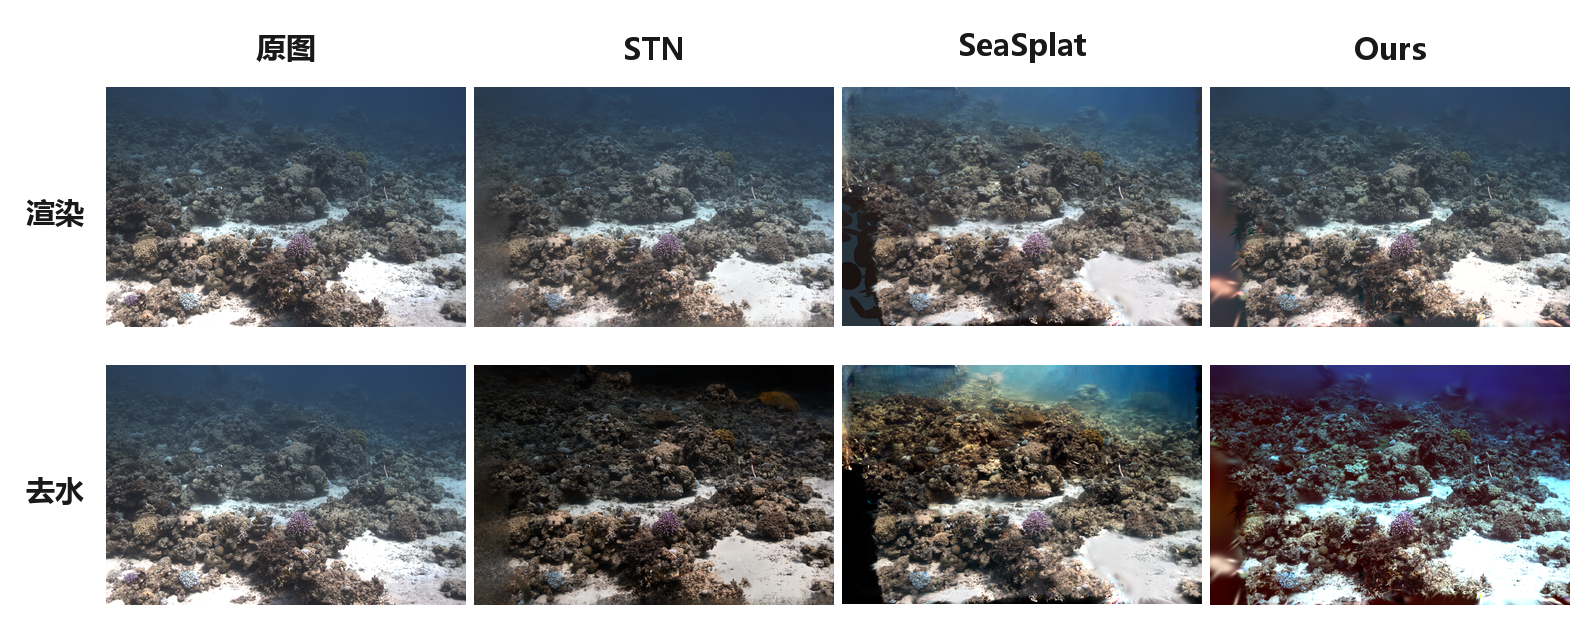
\includegraphics[width=\textwidth]{figures/static_multimethod/japanese_dewater_render_compare.png}
  \caption{JapaneseGardens-RedSea场景原图、渲染结果与去水结果对比。上行为带水渲染结果，下行为去水结果；原图列在两行中重复显示作为参考。}
  \label{fig:static_japanese_dewater}
\end{figure}

由表\ref{tab:psnr_static}可观察到，本文方法在JapaneseGardens-RedSea场景上的PSNR（23.38 dB）超过所有基线，相较SeaSplat提升+0.68 dB，相较4DGS提升+1.57 dB，反映出当场景具有丰富细粒度纹理时，本文方法的水下物理模型与深度监督相结合所带来的联合约束依然能够提供增益；相较于不带水下物理模型的原始4DGS\upcite{wu2024gaussian}，本文方法在所有四个静态场景上的PSNR平均提升约1.05 dB，且SSIM与LPIPS同步改善，表明所引入的水下物理建模能够在动态主干基础上有效补偿静态场景的色偏与散射；本文方法在Curaçao、IUI3-RedSea、Panama上仍略逊于SeaSplat，原因在于SeaSplat专为静态场景优化，而本文方法在这些场景中保留的形变场参数构成不必要的自由度，引入了一定的优化噪声。

此外，本文方法在SaltPond场景上的实验也作为额外的鲁棒性参考。在该场景上，仅使用深度监督而未启用水下优化的配置PSNR为26.11 dB（SSIM为0.6251）；启用完整水下优化后，本文方法PSNR提升至27.15 dB（SSIM为0.7036），相较原始SeaSplat论文报告的27.47 dB仅低0.32 dB。

\section{对比分析}

\subsection{与SeaSplat对比分析}

SeaSplat\upcite{seasplat2025icra}是面向静态场景设计的水下高斯溅射方法，其核心优势在于对水下色偏与散射的物理建模，但由于缺乏动态场景处理能力，其在动态数据集上的性能受到严重制约。

表\ref{tab:psnr_dynamic}中各场景的对比数据清晰地反映了这一局限。在Robot场景中，本文方法PSNR为29.71 dB，而SeaSplat仅为28.21 dB，提升约5.3\%；在Fish场景中，差距最为悬殊，本文方法（28.52 dB）相较于SeaSplat（23.30 dB）提升约22.4\%；在Coral场景中，提升幅度高达25.2\%（33.29 vs 26.58 dB）。

上述差距的原因在于，Fish场景中鱼体的快速游动、Coral场景中珊瑚枝条的持续摆动，以及Robot场景中机械臂的往复运动，均会导致多帧图像之间出现显著的非刚性形变。静态方法（包括SeaSplat）在处理此类输入时，无法将运动信息从场景几何中解耦，使得对应运动区域的高斯体在训练过程中接收到来自不同帧的矛盾监督信号，最终收敛至多帧叠加的模糊状态，导致渲染结果在运动区域出现严重的鬼影与模糊。相比之下，本文方法通过时间相关的形变场对运动进行显式建模，有效消除了上述模糊现象。

SeaSplat在Streaks场景（26.16 dB）上的劣势相对于其他两种静态方法（3DGS为26.47 dB）更为明显，这可能与水下光焦散的时变特性同其水下物理模型的静态假设之间的冲突有关，动态光纹被错误地纳入后向散射项建模，导致模型估计出错。

\subsection{与4DGS和UDR-GS对比分析}

\textbf{（1）Robot场景}

在Robot场景中，本文方法（29.71 dB）略优于4DGS（29.49 dB）和UDR-GS（29.62 dB），三者差距在0.3\%至0.7\%之间。机械臂运动具有规律性，三种动态方法均能较好地建模其运动轨迹，因此差距相对有限。本文方法在SSIM上的优势表明其对机械臂边缘的结构细节刻画更为精确，但LPIPS指标（0.1587）高于UDR-GS（0.0840），反映出在感知质量方面存在一定不足，可能与本文方法引入的水下颜色恢复模块改变了局部纹理的高频特征分布有关。

\textbf{（2）Fish场景}

Fish场景是本文方法的相对薄弱场景。鱼体的快速非规律性运动与颜色恢复模块之间存在梯度冲突：在快速运动区域，形变场的估计误差会导致颜色恢复模块接收到不一致的颜色监督信号，进而干扰水体参数的准确估计。UDR-GS（29.24 dB）由于不引入颜色恢复的额外参数，其优化目标更为单一，在此类高速运动场景下反而获得了更稳定的收敛。这一结果表明，如何在快速运动场景中降低多模块间的梯度干扰，是未来工作需要重点改进的方向之一。

\textbf{（3）Coral场景}

Coral场景最充分地体现了本文方法的综合优势。珊瑚礁场景同时具有动态性（珊瑚摆动）和显著的水下色偏（蓝绿色偏移），这正是本文方法所针对的双重挑战。本文方法PSNR（33.29 dB）相较UDR-GS（32.43 dB）提升+2.7\%，相较4DGS（31.14 dB）提升+6.9\%，SSIM也由0.9475提升至0.9640。这一结果印证了完整水下物理模型在恢复珊瑚礁真实色彩方面的重要作用：4DGS缺乏色彩校正，导致颜色失真使PSNR受损；UDR-GS虽具备一定的水下处理能力，但其颜色恢复能力弱于本文方法，因此在涉及色偏的质量指标上略逊。

\textbf{（4）Streaks场景}

Streaks场景展示了本文方法最显著的性能优势。水下光焦散产生的时变光纹不仅是一种动态现象，更与水体的光学散射特性密切相关。本文方法通过动态高斯建模捕捉光纹的时变形态，同时通过水下物理模型将光焦散的颜色特性与环境散射项解耦，两个模块形成协同效应。PSNR提升1.74 dB（从28.91至30.65 dB），SSIM提升8.1\%（从0.8648至0.9349），LPIPS降低31.5\%（从0.0883至0.0605），三项指标全面领先，充分验证了动态建模与水下物理建模联合设计的有效性。



\section{可视化结果}

\subsection{渲染效果对比}

图\ref{fig:render_compare}展示了本文方法与SeaSplat在四个动态场景上的渲染效果对比。每行对应一个动态水下场景（Robot、Coral、Fish、Streaks），每列从左至右依次为：测试视角采集到的原始水下参考图像（GT）、SeaSplat的渲染图像、SeaSplat的深度图（以热力图显示）、本文方法的渲染结果、本文方法的深度图（以热力图显示）。深度图颜色仅表示相对远近关系，不代表RGB渲染颜色。通过对比SeaSplat渲染图像与GT，可以观察到静态方法在动态区域容易出现重影与模糊；本文方法在运动区域的轮廓保持更稳定。

\begin{figure}[htbp]
  \centering
  \setlength{\tabcolsep}{1pt}
  \renewcommand{\arraystretch}{0.6}
  \begin{tabular}{@{}>{\centering\arraybackslash}m{1.2em}@{\hspace{2pt}}*{5}{>{\centering\arraybackslash}m{0.17\textwidth}}@{}}
     & GT（原始） & SeaSplat & SeaSplat深度 & 本文方法 & 本文深度 \\
    \rotatebox{90}{Robot}   & 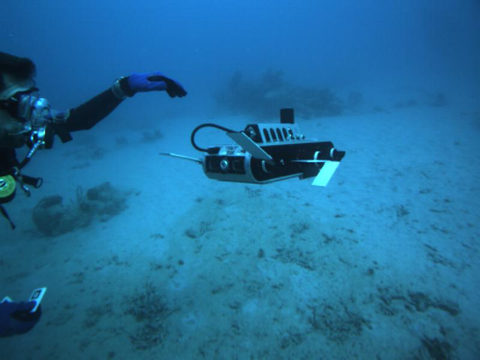
\includegraphics[width=0.17\textwidth]{figures/render_compare/robot_gt.png}   & 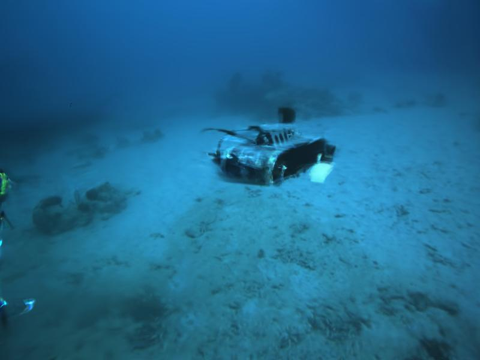
\includegraphics[width=0.17\textwidth]{figures/render_compare/robot_sea_water.png}   & 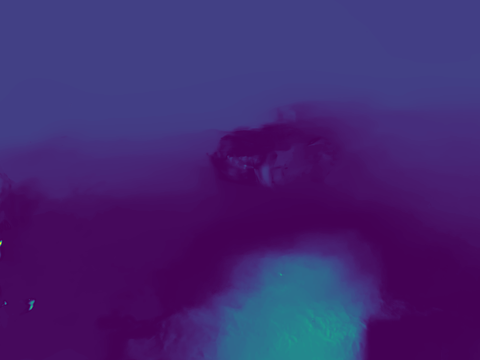
\includegraphics[width=0.17\textwidth]{figures/render_compare/robot_sea_depth.png}   & 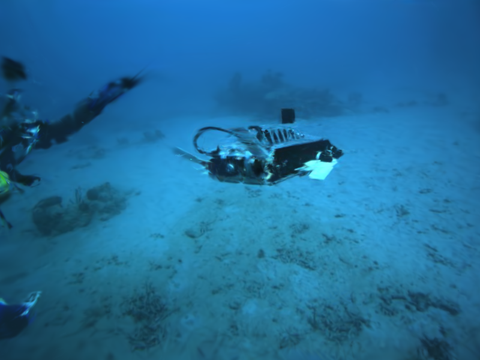
\includegraphics[width=0.17\textwidth]{figures/render_compare/robot_ours.png}   & 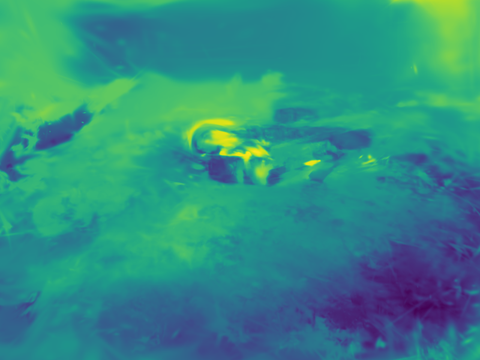
\includegraphics[width=0.17\textwidth]{figures/render_compare/robot_ours_depth.png}   \\
    \rotatebox{90}{Coral}   & 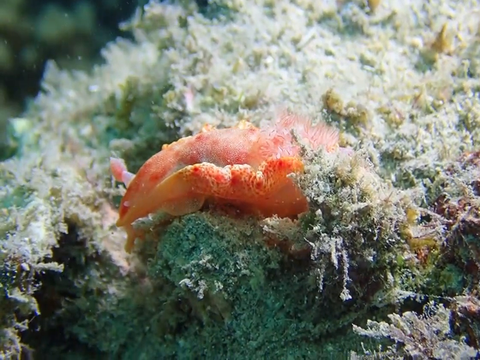
\includegraphics[width=0.17\textwidth]{figures/render_compare/coral_gt.png}   & 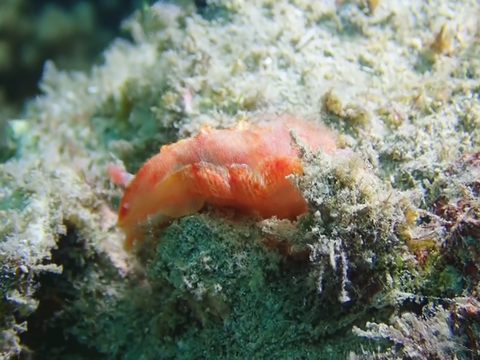
\includegraphics[width=0.17\textwidth]{figures/render_compare/coral_sea_water.png}   & 
\includegraphics[width=0.17\textwidth]{figures/render_compare/coral_sea_depth.png}   & 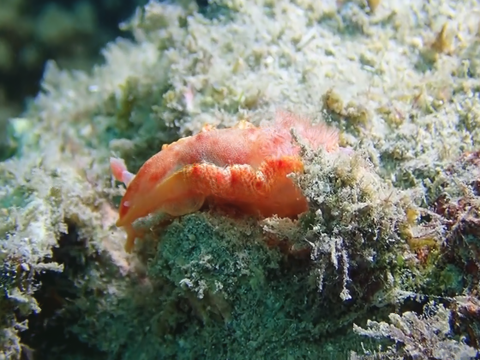
\includegraphics[width=0.17\textwidth]{figures/render_compare/coral_ours.png}   & 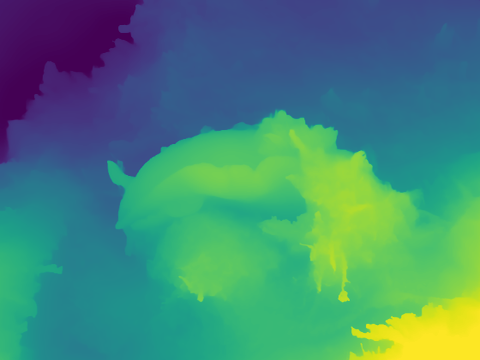
\includegraphics[width=0.17\textwidth]{figures/render_compare/coral_ours_depth.png}   \\
    \rotatebox{90}{Fish}    & \includegraphics[width=0.17\textwidth]{figures/render_compare/fish_gt.png}    & 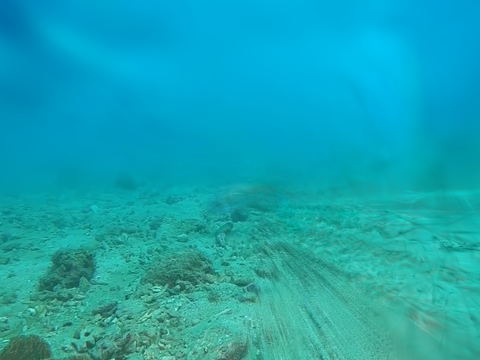
\includegraphics[width=0.17\textwidth]{figures/render_compare/fish_sea_water.png}    & 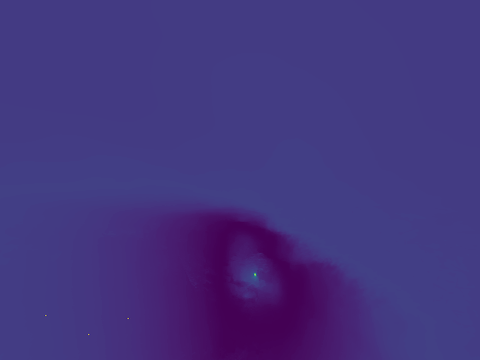
\includegraphics[width=0.17\textwidth]{figures/render_compare/fish_sea_depth.png}    & 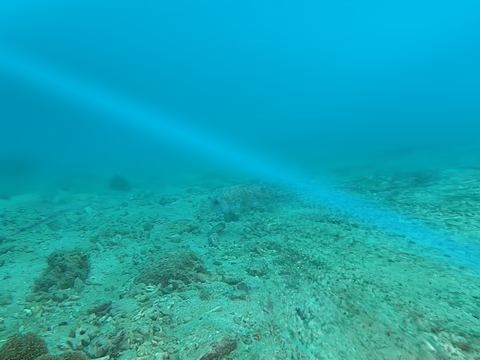
\includegraphics[width=0.17\textwidth]{figures/render_compare/fish_ours.png}    & 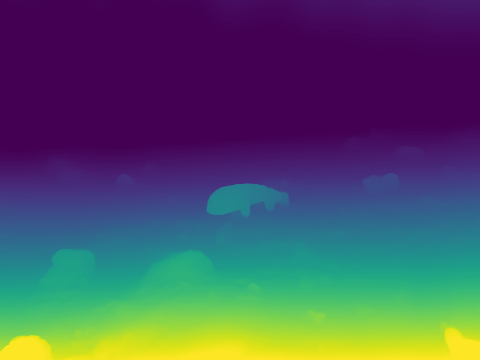
\includegraphics[width=0.17\textwidth]{figures/render_compare/fish_ours_depth.png}    \\
    \rotatebox{90}{Streaks} & \includegraphics[width=0.17\textwidth]{figures/render_compare/streaks_gt.png} & 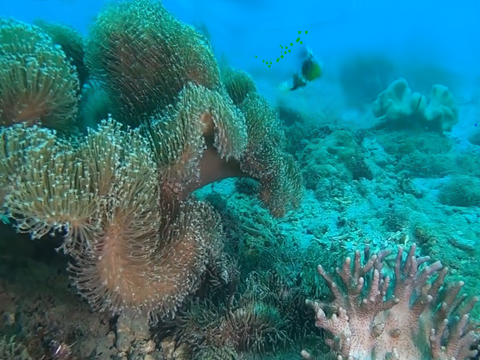
\includegraphics[width=0.17\textwidth]{figures/render_compare/streaks_sea_water.png} & 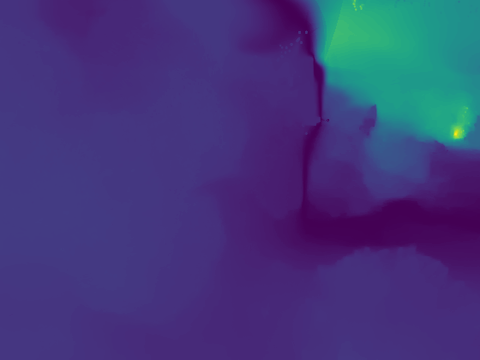
\includegraphics[width=0.17\textwidth]{figures/render_compare/streaks_sea_depth.png} & 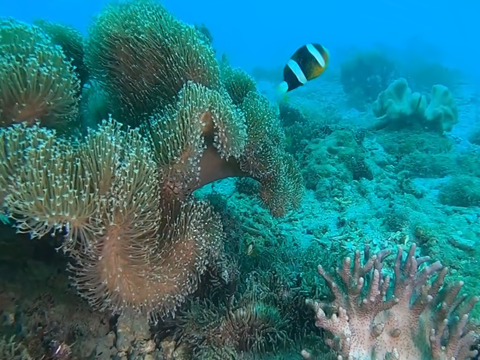
\includegraphics[width=0.17\textwidth]{figures/render_compare/streaks_ours.png} & 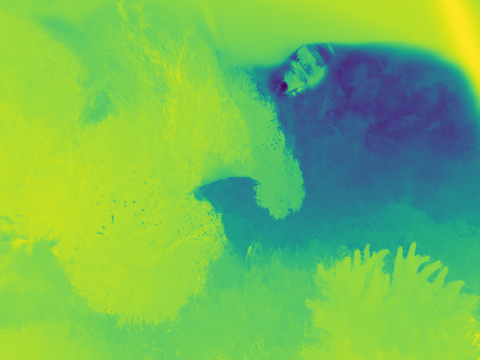
\includegraphics[width=0.17\textwidth]{figures/render_compare/streaks_ours_depth.png} \\
  \end{tabular}
  \caption{四个动态水下场景的渲染效果对比。GT为测试视角采集到的原始水下参考图像；两列深度图为相对深度的热力图显示。与SeaSplat静态基线相比，本文方法在动态区域的重影和轮廓模糊更少。}
  \label{fig:render_compare}
\end{figure}

由图\ref{fig:render_compare}可以观察到，在各个场景中，SeaSplat由于缺乏动态建模能力，在运动物体区域更容易出现重影与模糊；本文方法通过时变高斯形变场显式建模运动，使运动物体轮廓保持相对稳定。需要注意的是，图中深度结果主要用于辅助判断几何连续性，定量结论仍以表\ref{tab:psnr_dynamic}和表\ref{tab:multi_metric}为准。


\subsection{水下去水效果}

图\ref{fig:dewater}展示了本文方法在四个动态水下场景上的水下图像分解效果。每行对应一个场景，其中$\mathbf{I}$表示模型合成的水下观测图像，$\mathbf{J}$表示依据水下成像模型反演得到的干净外观图像，即$\mathbf{J}=(\mathbf{I}-\mathbf{B}(\mathbf{Z}))\oslash\mathbf{A}(\mathbf{Z})$（$\oslash$表示逐元素除法）。这里的"去水"不是额外的图像增强后处理，而是模型内部物理分解得到的外观项。

\begin{figure}[htbp]
  \centering
  \setlength{\tabcolsep}{2pt}
  \renewcommand{\arraystretch}{0.6}
  \begin{tabular}{@{}>{\centering\arraybackslash}m{1.2em}@{\hspace{2pt}}*{5}{>{\centering\arraybackslash}m{0.17\textwidth}}@{}}
     & GT（原始） & SeaSplat $\mathbf{I}$ & SeaSplat $\mathbf{J}$ & 本文 $\mathbf{I}$ & 本文 $\mathbf{J}$ \\
    \rotatebox{90}{Robot}   & 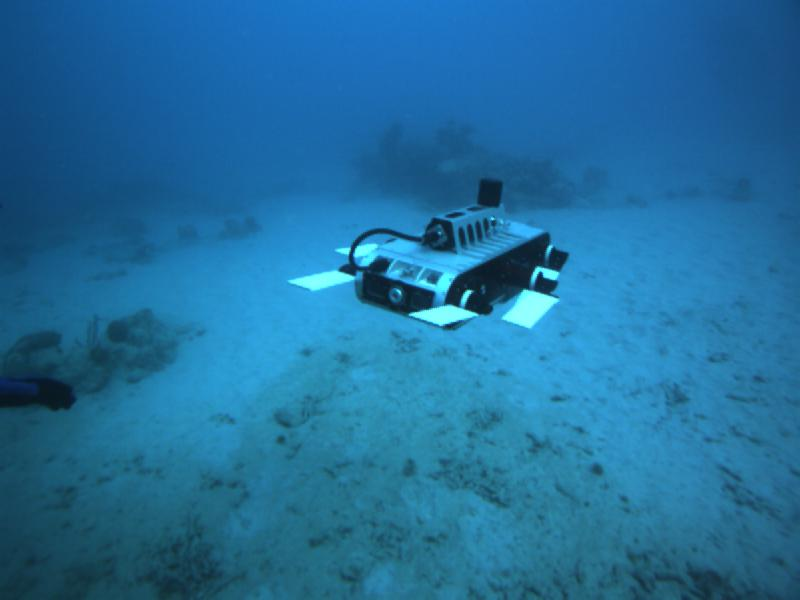
\includegraphics[width=0.17\textwidth]{figures/dewater/robot_gt.png}   & 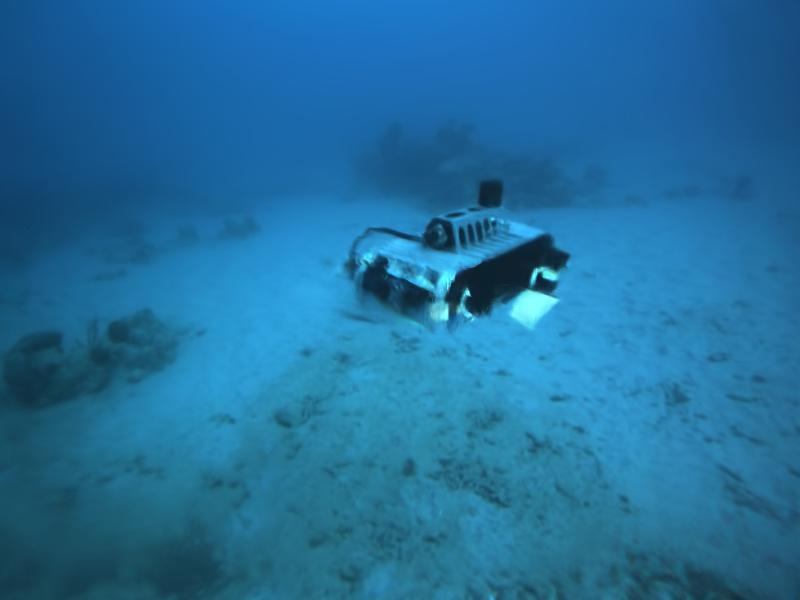
\includegraphics[width=0.17\textwidth]{figures/dewater/robot_sea_I.png}   & 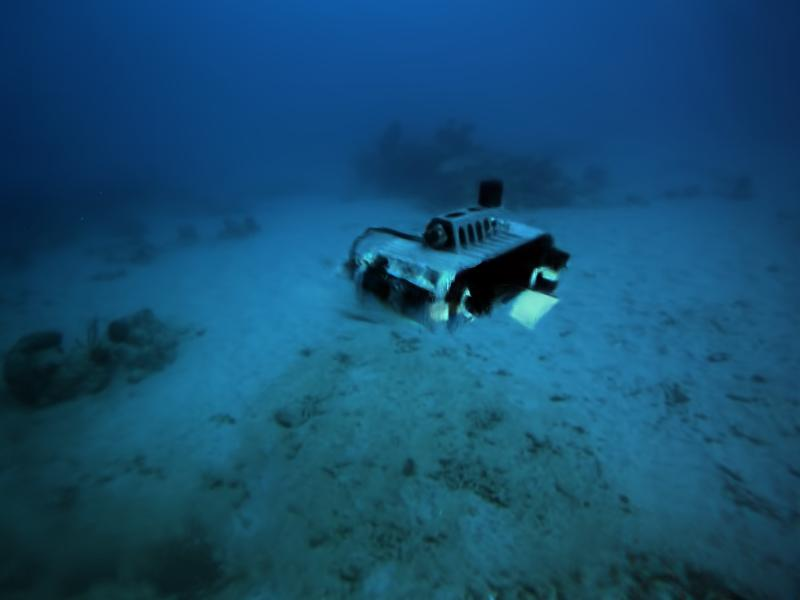
\includegraphics[width=0.17\textwidth]{figures/dewater/robot_sea_J.png}   & 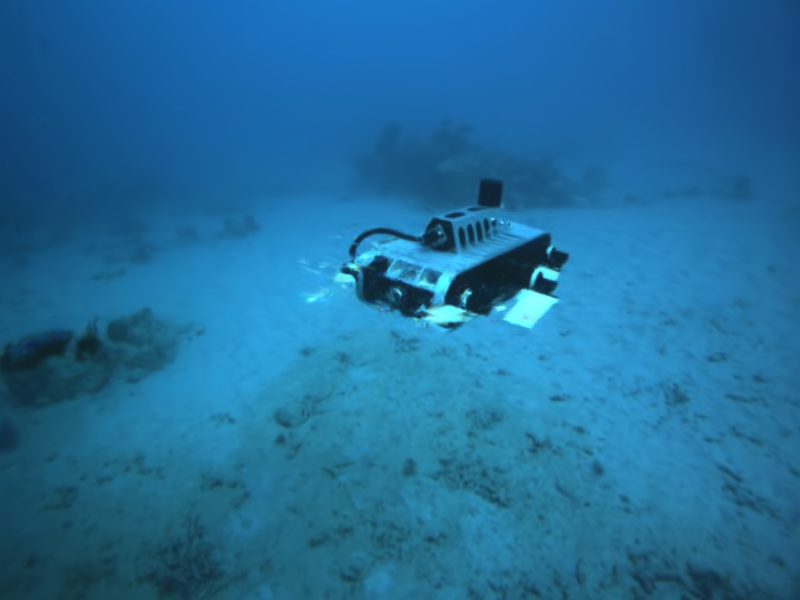
\includegraphics[width=0.17\textwidth]{figures/dewater/robot_ours_I.png}   & 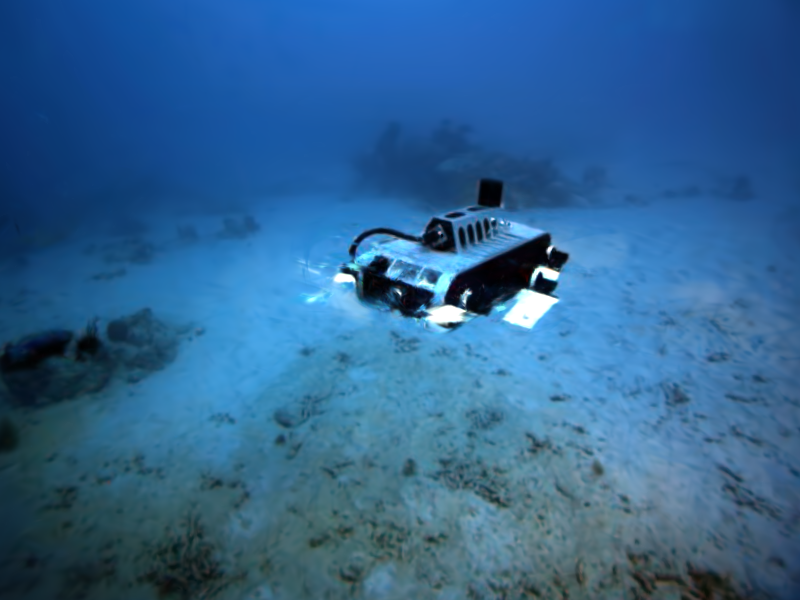
\includegraphics[width=0.17\textwidth]{figures/dewater/robot_ours_J.png}   \\
    \rotatebox{90}{Coral}   & 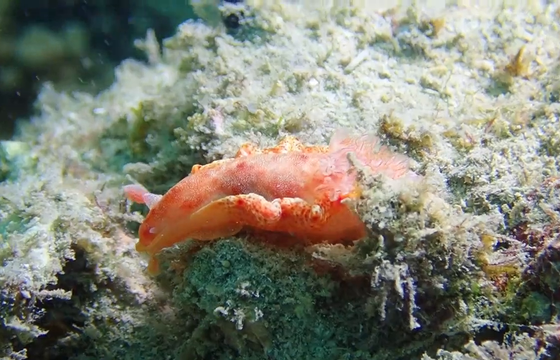
\includegraphics[width=0.17\textwidth]{figures/dewater/coral_gt.png}   & 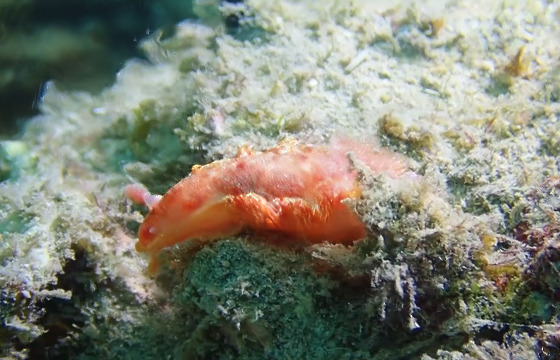
\includegraphics[width=0.17\textwidth]{figures/dewater/coral_sea_I.png}   & 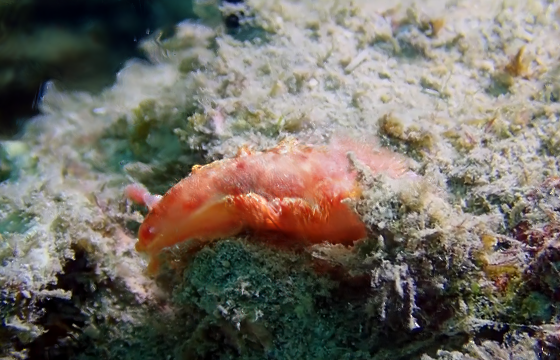
\includegraphics[width=0.17\textwidth]{figures/dewater/coral_sea_J.png}   & 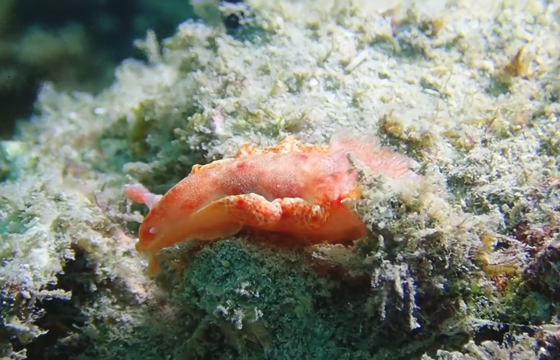
\includegraphics[width=0.17\textwidth]{figures/dewater/coral_ours_I.png}   & 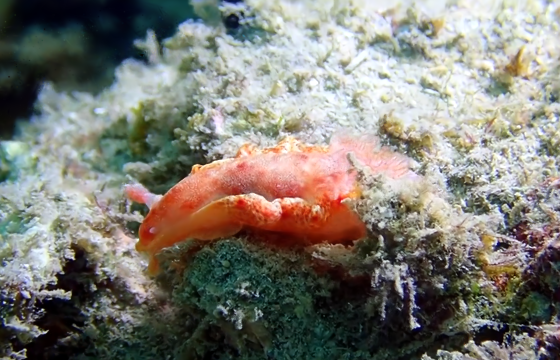
\includegraphics[width=0.17\textwidth]{figures/dewater/coral_ours_J.png}   \\
    \rotatebox{90}{Fish}    & \includegraphics[width=0.17\textwidth]{figures/dewater/fish_gt.png}    & 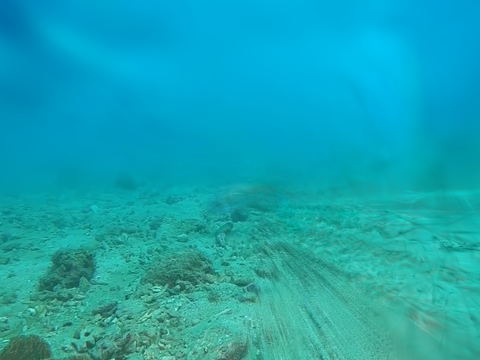
\includegraphics[width=0.17\textwidth]{figures/dewater/fish_sea_I.png}    & 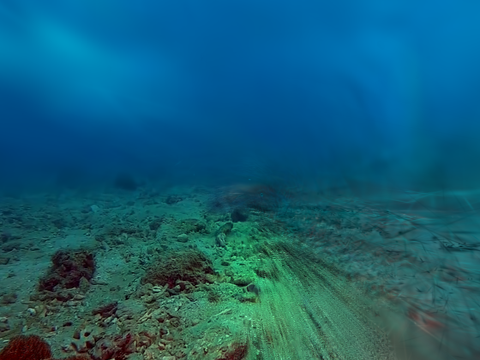
\includegraphics[width=0.17\textwidth]{figures/dewater/fish_sea_J.png}    & 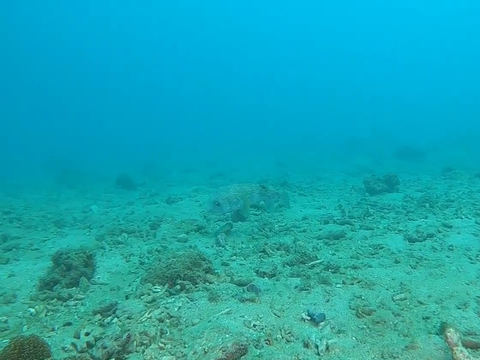
\includegraphics[width=0.17\textwidth]{figures/dewater/fish_ours_I.png}    & 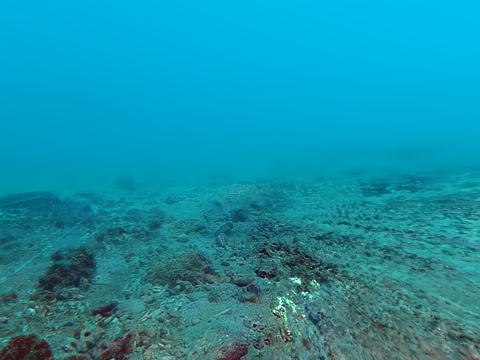
\includegraphics[width=0.17\textwidth]{figures/dewater/fish_ours_J.png}    \\
    \rotatebox{90}{Streaks} & 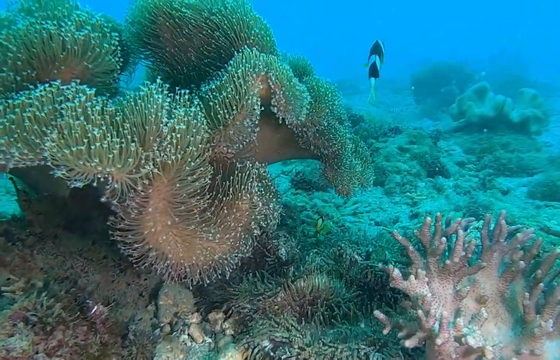
\includegraphics[width=0.17\textwidth]{figures/dewater/streaks_gt.png} & 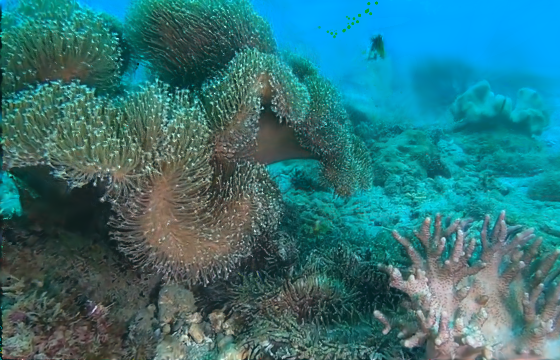
\includegraphics[width=0.17\textwidth]{figures/dewater/streaks_sea_I.png} & 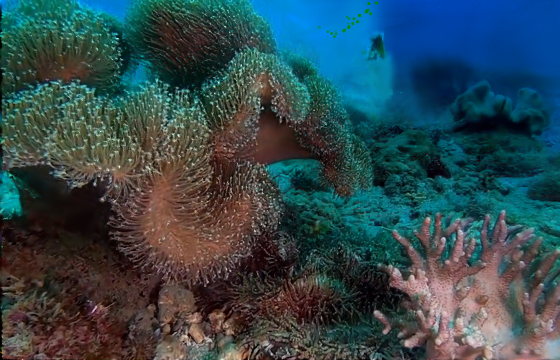
\includegraphics[width=0.17\textwidth]{figures/dewater/streaks_sea_J.png} & 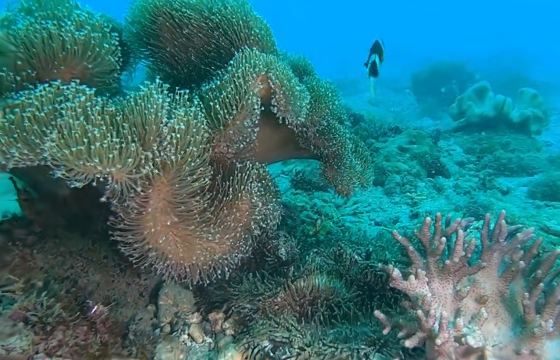
\includegraphics[width=0.17\textwidth]{figures/dewater/streaks_ours_I.png} & 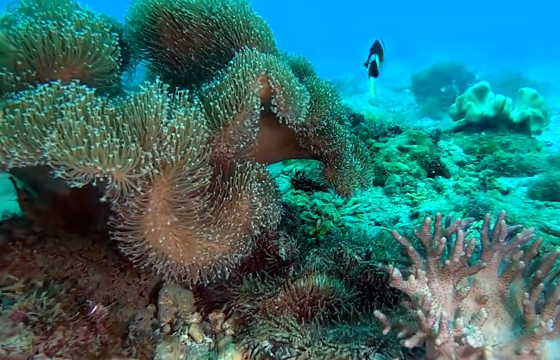
\includegraphics[width=0.17\textwidth]{figures/dewater/streaks_ours_J.png} \\
  \end{tabular}
  \caption{四个动态水下场景的物理分解结果。从左至右依次为：测试视角原始水下参考图像（GT）、SeaSplat渲染水下观测图像$\mathbf{I}$、SeaSplat反演干净外观$\mathbf{J}$、本文方法渲染水下观测图像$\mathbf{I}$、本文方法反演干净外观$\mathbf{J}$。}
  \label{fig:dewater}
\end{figure}

对比图中，本文$\mathbf{I}$与本文$\mathbf{J}$在部分场景下差异并不剧烈，这与两个因素有关：一方面，训练目标直接约束的是与GT一致的水下观测图像$\mathbf{I}$，物理反演项$\mathbf{J}$主要用于约束高斯外观而非追求主观增强效果；另一方面，Robot和Fish等场景的有效可见距离较短，学习到的衰减和后向散射幅度有限，因此反演前后的视觉差异相对温和。该图更适合说明模型是否形成了可解释的$\mathbf{I}/\mathbf{J}$分解，而不是作为传统水下图像增强算法的主观对比。

\subsection{中间产物可视化}

图\ref{fig:intermediate}展示了本文方法在四个动态水下场景上估计的中间产物。每行对应一个场景，从左至右依次为：原始输入图像、估计深度图$\mathbf{Z}$（以热力图显示）、衰减图 $\mathbf{A}(\mathbf{Z})$（按 $A_c(Z)=\exp(-\beta_c^D Z)$ 逐元素计算）以及后向散射估计 $\mathbf{B}(\mathbf{Z})$（按 $B_c(Z)=B_c^\infty\left(1-\exp(-\beta_c^B Z)\right)$ 逐元素计算），深度与水体参数图均采用viridis色图渲染。

\begin{figure}[htbp]
  \centering
  \setlength{\tabcolsep}{1pt}
  \renewcommand{\arraystretch}{0.6}
  \begin{tabular}{@{}>{\centering\arraybackslash}m{1.2em}@{\hspace{2pt}}*{4}{>{\centering\arraybackslash}m{0.21\textwidth}}@{}}
     & 输入图像 & 深度 $\mathbf{Z}$ & 衰减 $\mathbf{A}(\mathbf{Z})$ & 后向散射 $\mathbf{B}(\mathbf{Z})$ \\
    \rotatebox{90}{Robot}   & 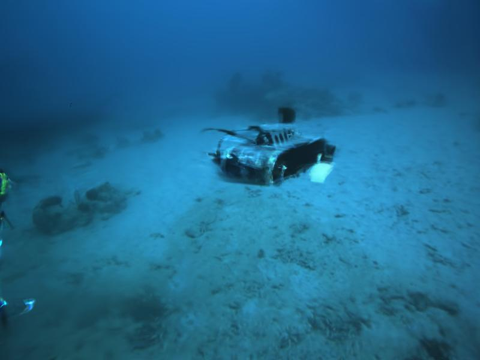
\includegraphics[width=0.21\textwidth]{figures/intermediate/robot_input.png}   & 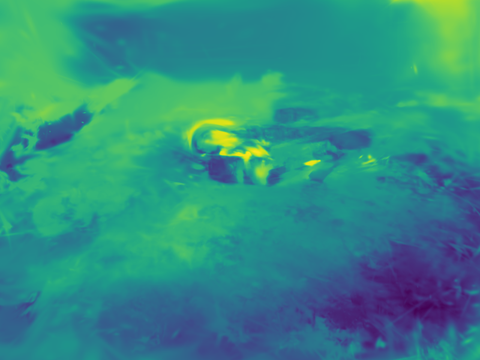
\includegraphics[width=0.21\textwidth]{figures/intermediate/robot_depth.png}   & 
\includegraphics[width=0.21\textwidth]{figures/intermediate/robot_atten.png}   & 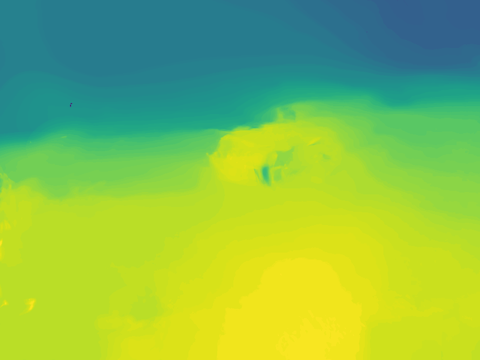
\includegraphics[width=0.21\textwidth]{figures/intermediate/robot_bs.png}   \\
    \rotatebox{90}{Coral}   & 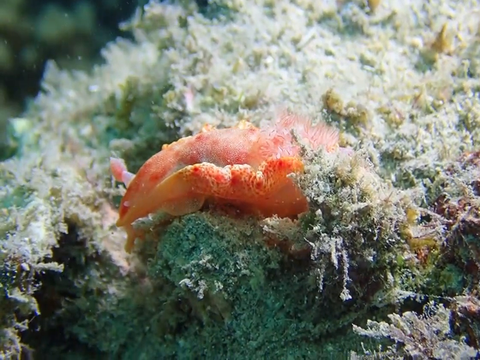
\includegraphics[width=0.21\textwidth]{figures/intermediate/coral_input.png}   & 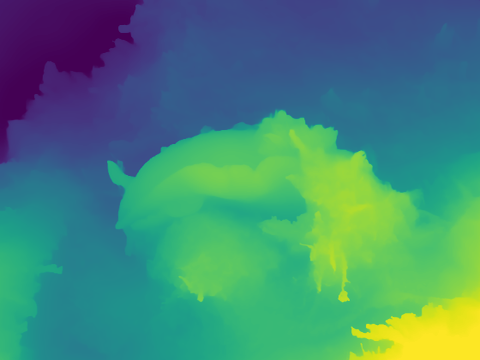
\includegraphics[width=0.21\textwidth]{figures/intermediate/coral_depth.png}   & 
\includegraphics[width=0.21\textwidth]{figures/intermediate/coral_atten.png}   & 
\includegraphics[width=0.21\textwidth]{figures/intermediate/coral_bs.png}   \\
    \rotatebox{90}{Fish}    & 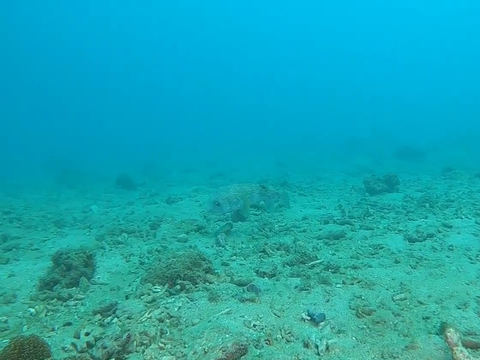
\includegraphics[width=0.21\textwidth]{figures/intermediate/fish_input.png}    & 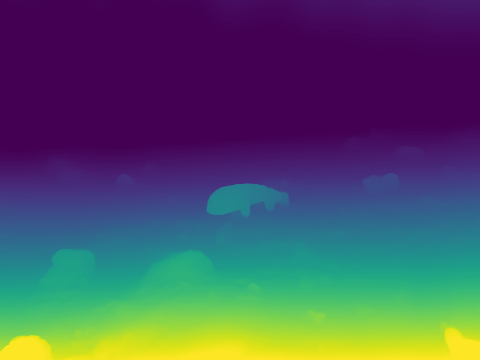
\includegraphics[width=0.21\textwidth]{figures/intermediate/fish_depth.png}    & 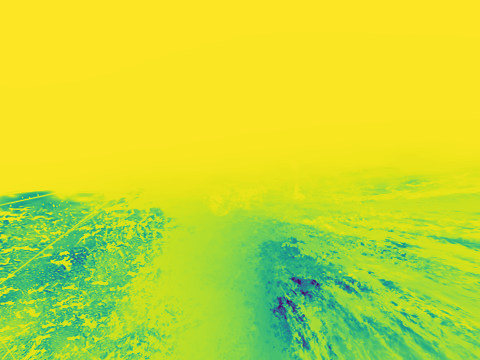
\includegraphics[width=0.21\textwidth]{figures/intermediate/fish_atten.png}    & 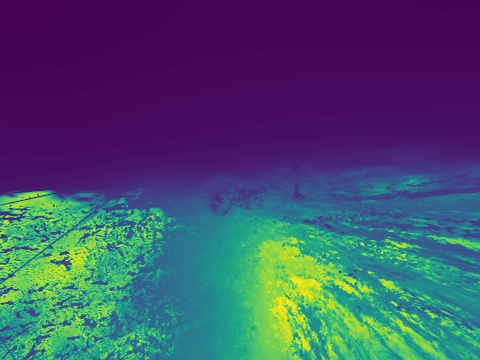
\includegraphics[width=0.21\textwidth]{figures/intermediate/fish_bs.png}    \\
    \rotatebox{90}{Streaks} & 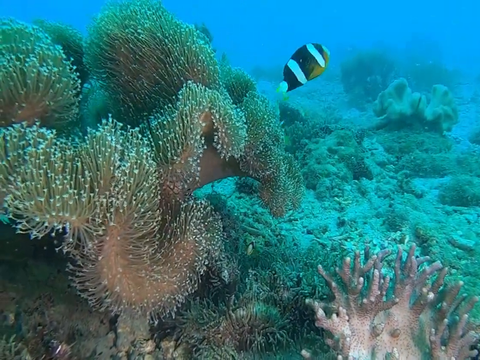
\includegraphics[width=0.21\textwidth]{figures/intermediate/streaks_input.png} & 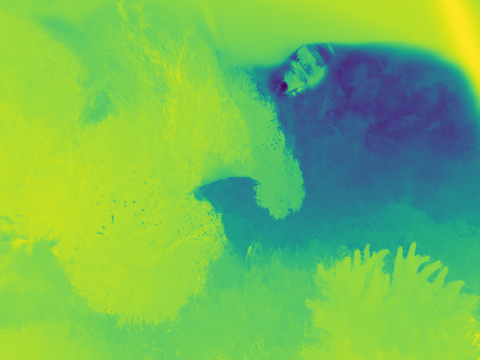
\includegraphics[width=0.21\textwidth]{figures/intermediate/streaks_depth.png} & 
\includegraphics[width=0.21\textwidth]{figures/intermediate/streaks_atten.png} & 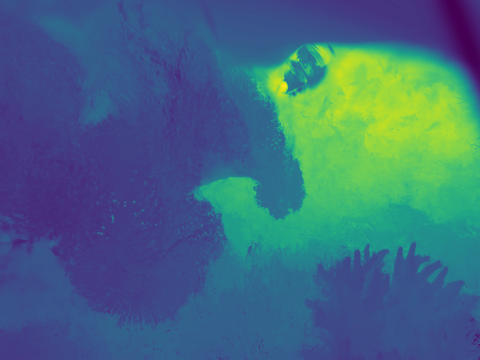
\includegraphics[width=0.21\textwidth]{figures/intermediate/streaks_bs.png} \\
  \end{tabular}
  \caption{四个动态水下场景的中间产物可视化。从左至右依次为：原始输入图像、估计深度图$\mathbf{Z}$、衰减图 $\mathbf{A}(\mathbf{Z})$（$A_c(Z)=\exp(-\beta_c^D Z)$ 逐元素）与后向散射 $\mathbf{B}(\mathbf{Z})$（$B_c(Z)=B_c^\infty(1-\exp(-\beta_c^B Z))$ 逐元素）。深度图采用热力图显示，仅表示相对远近关系。}
  \label{fig:intermediate}
\end{figure}

从图\ref{fig:intermediate}可以看出，估计深度图在主体物体轮廓和背景层次上保持了较连续的相对远近关系，说明单目深度监督对几何结构具有约束作用。衰减图$\mathbf{A}(\mathbf{Z})$在远景区域整体更低，后向散射图$\mathbf{B}(\mathbf{Z})$在较远区域通常更高，这与水下成像模型中"直接透射随距离衰减、后向散射随距离累积"的趋势一致。由于本文没有真实水体光学参数作为监督，上述中间产物只能作为物理趋势和可解释性的辅助证据，不能单独视为参数估计精度的严格验证。

\section{消融实验}

为系统评估本文方法中各核心组件的实际贡献，并揭示水下物理模型在不同场景特性下的适用边界，本文设计了组件解耦实验方案。本节将各场景置于相同硬件预算与相同初始化条件下，仅切换模型组件配置，从而准确隔离各模块的边际贡献。

\subsection{消融实验设计}

本文将完整模型分解为以下四种配置：

\begin{itemize}
  \item \textbf{（a）}仅保留时空高斯溅射主干，关闭水下物理模型与单目深度监督。
  \item \textbf{（b）}启用 SeaThru 物理模型（后向散射$\mathbf{B}(\mathbf{Z})$与衰减$\mathbf{A}(\mathbf{Z})$双子网络），但不引入深度监督。
  \item \textbf{（c）}仅启用基于 Depth Anything V2 的逆深度监督。
  \item \textbf{（d）}同时启用 SeaThru 物理模型与深度监督，即本文完整方法。
\end{itemize}

四种配置在 Robot、Fish、Coral、Streaks 四个动态场景上运行。

\subsection{定量结果}

表\ref{tab:ablation_psnr}给出了四种配置在四个场景上的 PSNR 定量结果。

\begin{table}[htbp]
  \centering
  \tablecaption{消融实验（PSNR / dB）}
  \label{tab:ablation_psnr}
  \begin{tabular}{lcccc}
    \hline
    \textbf{场景} & \textbf{a} & \textbf{b} & \textbf{c} & \textbf{d} \\
    \hline
    Robot   & 29.49               & 29.40                 & 29.24               & \textbf{29.71} \\
    Fish    & \textbf{29.09}      & 27.92     & 28.54               & 28.52 \\
    Coral   & 31.14               & 32.02     & \textbf{33.44}      & 33.29 \\
    Streaks & 28.81               & 30.50                 & \textbf{30.78}      & 30.65 \\
    \hline
  \end{tabular}
\end{table}

表\ref{tab:ablation_ssim_lpips}进一步给出 SSIM 与 LPIPS 指标，便于多维度评估。

\begin{table}[htbp]
  \centering
  \tablecaption{消融实验补充指标（SSIM$\uparrow$ / LPIPS$\downarrow$)}
  \label{tab:ablation_ssim_lpips}
  \begin{tabular}{lcccc}
    \hline
    \textbf{场景} & \textbf{a} & \textbf{b} & \textbf{c} & \textbf{d} \\
    \hline
    Robot   & 0.931 / \textbf{0.066} & 0.934 / 0.163 & 0.932 / 0.165 & \textbf{0.939} / 0.159 \\
    Fish    & 0.821 / 0.139 & 0.816 / 0.155 & 0.822 / 0.137 & \textbf{0.822 / 0.137} \\
    Coral   & 0.927 / 0.061 & 0.956 / 0.076 & \textbf{0.966} / 0.049 & 0.964 / \textbf{0.049} \\
    Streaks & 0.862 / 0.096 & 0.929 / 0.075 & \textbf{0.939} / 0.061 & 0.935 / \textbf{0.061} \\
    \hline
  \end{tabular}
\end{table}

由表\ref{tab:ablation_psnr}与表\ref{tab:ablation_ssim_lpips}可观察到，完整模型并非在所有场景上均为最优。完整模型在Robot上以29.71 dB取得最优PSNR；在Fish场景上，基础4DGS配置（29.09 dB）以约0.57 dB领先完整模型（28.52 dB）；在Coral与Streaks场景上，完整模型（33.29、30.65 dB）相较基础4DGS配置（31.14、28.81 dB）分别提升+2.15 dB和+1.84 dB。以下分析均以两张消融表的数值差异和图\ref{fig:ablation_qualitative}的可视化结果为依据，不额外假设未观测的水体参数。

\subsection{Robot 场景}

Robot场景中，完整模型的PSNR为29.71 dB，高于基础4DGS配置的29.49 dB，也高于仅引入水下物理模型配置的29.40 dB和仅引入深度监督配置的29.24 dB。该结果说明，在机械臂运动相对规则的情况下，单独加入一个组件并不一定带来稳定增益，但水下物理模型和深度监督共同使用时能够互相约束：深度监督减少几何漂移，水下物理模型则对颜色衰减和后向散射进行补偿。SSIM从基础配置的0.931提升至完整模型的0.939，也支持完整模型在结构保持上更稳定。

\subsection{Streaks 场景}

Streaks场景中，基础4DGS配置的PSNR为28.81 dB，仅引入水下物理模型后提升至30.50 dB，仅引入深度监督后进一步提升至30.78 dB，完整模型为30.65 dB。由此可见，两类组件均能改善该场景，但深度监督带来的增益更大；完整模型略低于仅深度监督配置0.13 dB，说明水下物理模型在该场景中并没有提供额外的正向叠加。

这一现象与Streaks场景的外观特征相符：该场景主要挑战是随时间变化的光纹和局部亮度条纹，而式\eqref{eq:uwmodel}中的后向散射项主要描述随深度累积的介质颜色贡献。若动态光纹被水下物理模型部分吸收为介质项，可能会削弱形变网络和深度监督对真实时变外观的表达。因此，在Streaks场景中，本文更倾向于将性能提升归因于深度监督带来的几何稳定性，而不是简单归因于完整水下物理模型。

\subsection{Coral 场景}

Coral场景中，基础4DGS配置的PSNR为31.14 dB，仅引入水下物理模型提升至32.02 dB，仅引入深度监督提升至33.44 dB，完整模型为33.29 dB。该结果说明，Coral场景对深度监督较为敏感，几何约束是主要增益来源；水下物理模型也带来一定提升，但与深度监督叠加后没有超过仅深度监督配置。考虑到Coral场景中珊瑚枝条细碎且存在缓慢摆动，单目深度先验可以直接约束枝条与背景之间的层次关系，因此对PSNR和SSIM的提升更明显。

\subsection{Fish 场景}

Fish场景中，基础4DGS配置取得29.09 dB，高于仅水下物理模型配置的27.92 dB、仅深度监督配置的28.54 dB和完整模型的28.52 dB。该结果表明，对于鱼体快速游动且遮挡变化明显的场景，额外物理分解和深度先验都可能受到动态区域不一致监督的影响。本文方法在该场景的LPIPS与仅深度监督配置接近，但PSNR没有超过基础4DGS，说明当前联合优化策略对高速非刚性运动仍不够稳健。

\subsection{消融实验综合分析}

综合四个场景可以看出，水下物理模型和深度监督的收益依赖场景条件，并不存在对所有场景都最优的固定配置。根据消融结果，本文将影响因素概括为三个维度：水体退化强度、外观变化是否主要由深度相关介质效应造成、运动复杂度。该划分仅用于解释实验现象：当运动较稳定且水体退化明显时，完整模型更容易获得收益；当高速非刚性运动或时变光纹占主导时，额外物理参数可能引入优化负担，需要更谨慎地设置损失权重和训练阶段。

图\ref{fig:ablation_qualitative}以Robot场景为例，给出四种消融配置的渲染效果以及对应的深度图。图中(a)--(d)四列与表\ref{tab:ablation_psnr}中的四种配置一一对应，用于辅助观察不同组件对场景外观与几何重建的影响。

% 红框工具宏：在图像归一化坐标 (0.30,0.20)-(0.70,0.65) 区域绘制红色矩形以突出差异。
% (0,0)=左下，(1,1)=右上；如需调整位置可直接修改本宏定义中的坐标。
\providecommand{\hlimg}[2]{%
  \begin{tikzpicture}[inner sep=0]
    \node[anchor=south west] (im) {\includegraphics[width=#1]{#2}};
    \begin{scope}[x={(im.south east)},y={(im.north west)}]
      \draw[red,very thick] (0.30,0.20) rectangle (0.70,0.65);
    \end{scope}
  \end{tikzpicture}%
}

\begin{figure}[htbp]
  \centering
  \setlength{\tabcolsep}{1pt}
  \renewcommand{\arraystretch}{0.6}
  \begin{tabular}{@{}>{\centering\arraybackslash}m{1.2em}@{\hspace{2pt}}*{4}{>{\centering\arraybackslash}m{0.21\textwidth}}@{}}
     &  &  &  &  \\
    \rotatebox{90}{渲染} & \hlimg{0.21\textwidth}{figures/ablation/a_plain_render.png}  & \hlimg{0.21\textwidth}{figures/ablation/b_seathru_render.png}  & \hlimg{0.21\textwidth}{figures/ablation/c_depthonly_render.png}  & \hlimg{0.21\textwidth}{figures/ablation/d_full_render.png}  \\
    \rotatebox{90}{深度} & \hlimg{0.21\textwidth}{figures/ablation/a_plain_depth.png}   & \hlimg{0.21\textwidth}{figures/ablation/b_seathru_depth.png}   & \hlimg{0.21\textwidth}{figures/ablation/c_depthonly_depth.png}   & \hlimg{0.21\textwidth}{figures/ablation/d_full_depth.png}   \\
     & (a) & (b) & (c) & (d) \\
  \end{tabular}
  \caption{消融实验定性结果（Robot场景），红框标出各配置间差异最显著的区域。各列对应不同消融配置：(a)仅保留时空高斯溅射主干；(b)在(a)之上启用SeaThru水下物理模型；(c)在(a)之上仅启用基于Depth Anything V2的逆深度监督；(d)同时启用SeaThru物理模型与深度监督，即本文完整方法。上行为渲染结果，下行为对应深度图，下标(a)--(d)按老师建议置于图下。}
  \label{fig:ablation_qualitative}
\end{figure}

\subsection{分阶段训练策略消融实验}

为验证实验流程中分阶段训练设计的作用，本节围绕完整流程中的三个关键环节进行消融：粗训练阶段、SeaThru物理分支预热阶段，以及fine阶段初始的高斯参数短暂冻结。完整流程首先在0--3000次迭代中仅优化4D高斯表示，不启用SeaThru物理模型；进入fine阶段后，用学习到的背景初始化后向散射无穷远项，并短暂冻结非颜色高斯参数；随后进行1000次BackscatterNet/AttenuateNet预热、2000次高斯颜色调整，最后进入高斯表示与水下物理分支的间歇联合优化。

参考实验流程消融记录，本文在Robot、Fish、Coral、Streaks四个动态场景上比较不同训练配置。由于部分失败配置的后处理渲染结果存在空白帧或NaN高斯导致的渲染失败，本节不再使用这些不可靠图像作为定性对比，主要依据训练日志、测试集PSNR和稳定性记录进行分析。

\subsubsection{实验配置}

表~\ref{tab:ablation_training_config}给出了本节比较的训练流程配置。0 warmup用于检验物理分支预热是否必要；200 iter与500 iter warmup用于观察最短稳定预热长度；跳过coarse阶段用于验证几何初始化的重要性；取消短暂冻结则用于区分freeze机制与预热机制的相对贡献。

\begin{table}[htbp]
  \centering
  \tablecaption{训练流程消融配置}
  \label{tab:ablation_training_config}
  \small
  \begin{tabular}{p{0.24\textwidth}p{0.22\textwidth}p{0.40\textwidth}}
    \hline
    \textbf{配置} & \textbf{被移除或缩短的环节} & \textbf{实验目的} \\
    \hline
    0 warmup & 移除coarse、预热和freeze & 检验从第1次迭代同时优化高斯、BS/AT与深度监督是否稳定 \\
    200 iter warmup & 移除coarse，仅保留极短预热 & 检验少量预热能否避免立即崩溃 \\
    500 iter warmup & 将coarse与SeaThru开启提前到500次迭代附近 & 检验较短预热在不同场景上的稳定性边界 \\
    跳过coarse，保留完整预热 & 移除0--3000次高斯几何初始化 & 单独检验coarse阶段对几何与后续物理优化的影响 \\
    取消短暂freeze & 保留默认coarse与预热，仅取消fine初始冻结 & 检验freeze是否为主要稳定来源 \\
    \hline
  \end{tabular}
\end{table}

\subsubsection{定量结果}

表~\ref{tab:ablation_training_psnr}汇总了各配置的代表性测试集PSNR。对于训练能够完成但后处理渲染失败的配置，表中采用训练过程中保存的测试集评估值；对于发生CUDA错误或后处理失败的配置，在稳定性列中单独说明。

\begin{table}[htbp]
  \centering
  \tablecaption{训练流程消融实验结果（PSNR / dB）}
  \label{tab:ablation_training_psnr}
  \small
  \begin{tabular}{p{0.25\textwidth}ccccp{0.19\textwidth}}
    \hline
    \textbf{训练配置} & \textbf{Robot} & \textbf{Fish} & \textbf{Coral} & \textbf{Streaks} & \textbf{稳定性摘要} \\
    \hline
    0 warmup & 14.62 & 13.30 & 10.75 & 13.57 & 全部场景持续NaN或停滞 \\
    200 iter warmup，无coarse & 25.98 & 26.68 & 13.82 & 20.58 & 可避免部分崩溃，但Fish后处理渲染失败，Coral质量较低 \\
    500 iter warmup & 26.35 & 26.63 & 19.24 & 19.75 & 训练稳定，但复杂场景质量仍受限 \\
    跳过coarse，保留完整预热 & 28.69 & 18.71 & 6.82 & 10.96 & Robot可训练，其余场景明显退化或崩溃 \\
    取消短暂freeze & 28.11 & 26.77 & 23.57 & 20.21 & 整体稳定，说明freeze不是主要瓶颈 \\
    \hline
  \end{tabular}
\end{table}

从表~\ref{tab:ablation_training_psnr}可以看出，完全取消预热会使四个场景的PSNR均跌至10--15 dB区间，训练日志中伴随长时间NaN梯度警告或训练停滞。200次迭代的极短预热能够降低立即崩溃的概率，例如Fish训练过程中的测试PSNR可恢复到26 dB以上，但后处理渲染仍可能因为NaN高斯失败；Coral场景PSNR仅为13.82 dB，说明极短预热只能缓解数值崩溃，并不能保证复杂场景的几何与物理分解质量。500次迭代预热在四个场景上均能稳定完成训练，但Coral与Streaks仍明显低于理想结果，表明“稳定训练”和“充分重建质量”并不等价。

跳过coarse阶段的结果进一步说明，粗训练提供的几何初始化是复杂场景收敛的前提。Robot场景规模较小、运动和结构相对简单，即使移除coarse阶段仍可保持28 dB以上的PSNR；但Fish、Coral和Streaks在相同设置下分别降至18.71 dB、6.82 dB和10.96 dB，其中Streaks在fine初期曾达到较高PSNR，随后在水下物理分支介入后快速崩溃。这说明coarse阶段并非只提升初始指标，而是在后续SeaThru物理建模中提供稳定几何基础。

\subsubsection{稳定性分析}

表~\ref{tab:ablation_training_stability}给出了训练稳定性的日志摘要。这里不再简单统计最终是否完成训练，而是区分“训练完成但后处理失败”“训练中发生CUDA错误”和“训练完成但质量崩溃”等情况。

\begin{table}[htbp]
  \centering
  \tablecaption{训练流程消融实验稳定性摘要}
  \label{tab:ablation_training_stability}
  \small
  \begin{tabular}{p{0.24\textwidth}p{0.64\textwidth}}
    \hline
    \textbf{训练配置} & \textbf{日志现象} \\
    \hline
    0 warmup & Robot在1269--19994次迭代持续NaN；Fish、Coral、Streaks也出现长段连续NaN，部分早期实验直接停滞或崩溃。 \\
    200 iter warmup，无coarse & Robot无NaN且训练评估较好；Fish可完成训练但后处理渲染失败；Coral避免CUDA崩溃但PSNR仍低；Streaks可训练但质量有限。 \\
    500 iter warmup & 四个场景训练过程稳定，无明显NaN警告；但复杂场景仍需要更完整的coarse-to-fine流程才能获得更好的最终质量。 \\
    跳过coarse，保留完整预热 & Robot基本稳定；Fish出现大量NaN警告，Coral质量严重退化，Streaks出现由高PSNR到低PSNR的后期崩溃。 \\
    取消短暂freeze & 在默认coarse与预热保留时整体稳定，说明短暂冻结主要起辅助缓冲作用，核心稳定性来自coarse阶段与BS/AT预热。 \\
    \hline
  \end{tabular}
\end{table}

上述结果表明，训练流程中最关键的不是单一的参数开关，而是优化顺序。若一开始同时更新高斯几何、动态变形、BackscatterNet、AttenuateNet以及单目深度监督，多个分支会在几何尚未成形时相互补偿，导致梯度尺度失控。SeaThru预热先让BS/AT在相对固定的渲染输入上学习水下成像残差，coarse阶段则为后续物理分支提供可解释的场景几何。二者结合后，后续的颜色调整与间歇联合优化才有稳定基础。

\subsubsection{实验结论}

训练流程消融实验得到以下结论：
\begin{enumerate}
  \item \textbf{SeaThru预热是稳定训练的必要条件}：0 warmup在所有场景上都导致严重NaN或训练停滞，说明水下物理分支不能与未成形的高斯几何从第1次迭代开始强耦合优化。
  \item \textbf{coarse阶段对复杂动态场景不可替代}：Robot可以在无coarse设置下维持较高PSNR，但Fish、Coral和Streaks明显退化，说明粗训练主要解决复杂场景的几何稳定性，而不是简单增加训练迭代数。
  \item \textbf{短预热只能解决部分数值问题}：200或500次迭代预热可以降低崩溃概率，但不能保证复杂场景的最终质量；完整流程仍需要较充分的coarse-to-fine优化。
  \item \textbf{短暂freeze是辅助机制}：在默认coarse和预热保留时，取消fine初始的短暂freeze仍可稳定训练，说明本文流程的核心贡献来自分阶段优化顺序，而非单独依赖冻结操作。
\end{enumerate}

\subsubsection{对水下物理模型中间产物的影响}

训练流程还会影响深度图、去水图、后向散射图和衰减图等中间产物。图~\ref{fig:intermediate}展示了完整流程下各场景的中间产物。在0 warmup或跳过coarse的配置中，由于几何尚未稳定便开始强制拟合水下物理分支，BackscatterNet和AttenuateNet容易把几何误差解释为介质散射或透射衰减，最终表现为深度不连续、去水颜色异常、后向散射数值失真以及衰减图过暗或过亮。

相比之下，完整流程先建立相对稳定的4D高斯几何，再让BS/AT分支预热并进入间歇联合优化，使物理分支学习到的后向散射与直接透射更符合水下成像趋势。因此，分阶段训练不仅提升最终渲染PSNR，也决定了水下物理分解结果是否具有可解释性。

\chapter{总结与展望}

\section{工作总结}

本文针对水下动态场景的新视角合成问题，将水下物理建模与动态高斯溅射框架相结合，提出了统一的重建系统。主要工作包括：

（1）将SeaSplat的水下物理建模模块（衰减网络、后向散射网络及损失函数）集成至4DGaussians框架，实现对水下光学退化与动态场景变化的联合处理。

（2）实现基于Depth Anything V2的单目深度监督机制，通过逆深度归一化与alpha加权损失提升几何一致性，抑制浮游点云伪影。

（3）设计多阶段渐进式训练策略，通过独立水下优化器、后向散射与前向衰减参数预热、后向散射与前向衰减参数与高斯参数交替更新缓解多模块协同训练的梯度冲突，提升训练稳定性。

实验表明，本文方法在四个动态水下场景上平均PSNR达30.54 dB，较UDR-GS提升1.6\%，较4DGS提升3.1\%。其中Robot、Coral和Streaks场景取得最优PSNR，Fish场景仍受高速非刚性运动影响，说明当前物理建模与动态形变的联合优化仍存在改进空间。

\section{未来工作}

未来可从以下几个方面继续改进：

（1）\textbf{自适应训练调度}。当前训练的阶段切换时机和交替更新频率是人为设定的固定值，换一个场景可能需要重新调整。一个可行的思路是根据训练过程中的梯度变化或验证集上的重建误差来自动决定何时切换阶段、以及水下模块与高斯模块的更新频率比例，从而减少手动调参的工作量。

（2）\textbf{时序信息的利用}。本文目前对每帧图像独立进行处理，没有显式利用相邻帧之间的运动关联。Fish场景的结果表明，当鱼体运动较快时，水下物理模块与变形模块之间会产生一定的优化冲突。一个可能的改进方向是加入光流等时序约束，让相邻帧之间共享一部分运动信息，帮助系统在快速运动区域更稳定地估计水体参数。

（3）\textbf{更精细的物理模型}。当前的水下成像模型假设整个场景范围内的水体光学参数是均匀的，没有考虑实际水体可能存在分层或局部浑浊的情况。后续可以将逐通道的固定衰减系数改为随空间位置变化的形式，使其能够适应更复杂的水下环境。此外，如果能够获取偏振或光谱信息，也可以将现有的RGB三通道模型扩展为更丰富的多光谱模型。

（4）\textbf{水下场景专用的深度估计}。本文使用的Depth Anything V2虽然在通用场景上表现不错，但其训练数据以陆地场景为主，对水下散射模糊、低对比度区域的深度估计效果还有提升空间。后续可以收集水下双目或结构光数据对其进行微调，或者尝试将深度估计网络和高斯渲染管线一起训练，让深度估计随场景重建的改善而更新。

（5）\textbf{推理速度优化}。当前系统的推理时间主要由变形网络前向计算、水下网络逐像素处理以及高斯光栅化三步构成，还达不到水下机器人实时导航的要求。可以从几个方面入手：剪除对渲染贡献不大的冗余高斯点、压缩变形MLP的结构、将水下物理模型简化为更轻量的计算形式。如果条件允许，还可以尝试将整个渲染流程部署到NVIDIA Jetson等嵌入式计算平台上，利用TensorRT等工具进行推理加速。

（6）\textbf{更多场景下的验证与快速适配}。目前仅在四个动态水下场景和四个静态水下场景上进行了测试，后续需要在更广泛的水下环境中验证方法的稳定性，例如高浑浊的近岸水域、深海弱光环境、不同水色类型的水域等。此外，还可以尝试让系统在遇到新场景时，仅利用场景自身的重建误差对水下物理模型做少量迭代微调，使其快速适应新场景的水体特性，而不需要重新进行完整训练。

% -*- coding: utf-8 -*-

\zihaowu
\printbibliography[category=cited,title={参考文献}]

\end{spacing}

\end{document}
